\documentclass[conference]{IEEEtran}
\usepackage[T1]{fontenc}
\usepackage[utf8]{inputenc}
\usepackage{amsmath,amssymb,booktabs,array,longtable,tabularx,xurl,tikz,graphicx}
\usetikzlibrary{arrows.meta,positioning,plotmarks,patterns}
\usepackage{placeins}
\usepackage[hidelinks]{hyperref}
\setlength{\emergencystretch}{1em}
% Float placement policy only: no change to type size, leading, column width or margins.
\renewcommand{\topfraction}{0.92}
\renewcommand{\bottomfraction}{0.60}
\renewcommand{\textfraction}{0.07}
\renewcommand{\floatpagefraction}{0.75}
\renewcommand{\dbltopfraction}{0.92}
\renewcommand{\dblfloatpagefraction}{0.75}
\setcounter{topnumber}{3}
\setcounter{dbltopnumber}{3}
\setcounter{totalnumber}{4}
\begin{document}
\title{RealDefect-R: Replaying Well-Formed but Wrong Data in Shared Robot-Data Pipelines}
\maketitle
\begin{abstract}

Shared robot data can be well-formed but wrong: specified local checks can pass while physical meaning or temporal identity is incorrect, and a receiving party may lack the reference information needed to verify these meanings. RealDefect-R binds eight public defect histories from five ecosystems to pinned sources, verified input identities, executable decision rules, execution scopes and retained outcomes. Six paired mechanism replays and one converter-coverage audit meet their local rules; a normalization repair restores coverage but remains outside its numerical tolerance in 24 of 44 conditions. Across cases, correctness depends on coefficient conventions, calibration anchors, temporal correspondence, cross-layer identity and population references. Expressing the rules in Great Expectations separates all seven eligible artifact pairs, while declared-schema checks separate one, providing evidence of rule portability. At collection scale, a complete audit of a cross-organizational re-release finds 61,502 of 71,907 episode summaries inconsistent with collection identifiers, although four stated frame constraints pass and a separately versioned row-wise index check finds zero violations across 22,412,712 frames. All 71,907 records satisfy the seven tested prefix-local identity-summary relations; global agreement occurs only in the source group whose local and global counters coincide. A scoped metadata-update replay on four preselected records propagates the two affected records' discrepancies; a summary-only correction clears the targeted violations. These results make reference information and execution scope explicit, supporting auditable verification across data hand-offs.\par

\end{abstract}

\begin{IEEEkeywords}
data provenance, data versioning, reproducibility, shared data pipelines, robot learning datasets, defect corpus, data validation, dataset verification, replay
\end{IEEEkeywords}

\section{Introduction}

Robot-learning datasets can be produced, transformed and consumed by different parties: laboratories record demonstrations, framework maintainers convert them between formats and versions, publishers re-release them under a new name, and downstream teams train on the result. Correctness in such a shared pipeline extends beyond readability. A stage can emit values that are readable, correctly typed, in range and internally consistent even though the physical quantity or temporal identity they denote has changed; the next consumer inherits the new meaning with the old schema. OpenPI, for example, provides vision-language-action policies and a DROID training pipeline \cite{26}, and the release checks studied here concern the data hand-offs that supply such policies. We study well-formed but wrong artifacts: those that satisfy the stated local checks while violating a case-specific semantic relation.\par

A cross-organizational re-release illustrates this problem. In a pinned Cosmos3-DROID release---NVIDIA's conversion of the multi-institution DROID dataset to LeRobot v3.0---global episode boundaries, declared counts and camera interval chains are coherent, and four stated constraints on the identity columns of all 22,412,712 frames hold without exception. Yet 61,502 of its 71,907 per-episode summaries report identifiers from the source group's local numbering rather than the collection they now live in. This discrepancy matters to consumers because a compatible released merge path offsets exactly those fields on the assumption that they are global. The discrepancies thus concern relations between episode summaries and collection identifiers, despite the four passing frame-column constraints.\par

The same gap appears at the level of a single value in an Isaac Lab repair that changes a grasp offset from a scalar-first quaternion convention to a scalar-last one. Both arrays have four finite components and unit norm, and the old array is \textit{literally equal} to its source. Under the new convention, the array gives a rotation 120 degrees away from the intended offset \cite{1}; the stored coefficients do not record which convention produced them.\par

Although public issue trackers document many such failures, a URL alone is insufficient for reuse. Reuse requires the source version, the identity of the inputs read, the historical calculation exercised, the reference information on which the verdict depends, the complete decision rule, and its execution scope. RealDefect-R supplies that chain for eight cases and preserves the measured outcomes, including one that fails. It makes three contributions.\par

\begin{itemize}

\item \textbf{A replayable evidence resource and its protocol.} Eight public histories across five ecosystems, bound to pinned sources, inputs verified at a stated granularity, case-specific reference information, executable rules, execution-scope labels, original results and a retained negative case. The protocol is part of the resource because it makes each row of Table I checkable.

\item \textbf{Observed reference requirements, and rule portability.} Comparing the replays makes explicit the reference information each rule uses, whether supplied externally or read from another part of the same release. Running those rules natively in a pinned general-purpose validator then separates their faulty artifacts, exposing the reference dependencies needed to instantiate executable checks.

\item \textbf{A collection-scale consistency audit.} A complete audit of the Cosmos3-DROID release, reported in separated layers: a measured summary-layer disagreement, checked frame-level constraints with no failures, a controlled consumer consequence, and an explicitly unmeasured downstream effect.

\end{itemize}

Sections III-IV connect the case evidence to executable reference requirements; Section V tests cross-layer consistency in a shared re-release.\par

\section{Problem Setting and Research Questions}

Let \(A\) be the artifact a pipeline stage receives, \(T_v\) the versioned software that transforms it, and \(B = T_v(A)\) its published output. A consumer applies a local check \(S_c(X_c)\)---shape, dtype, finiteness, range, readability or internal consistency---to stated fields \(X_c\), which may be inputs or outputs. RD5, for example, distinguishes a normalized input action from the transformed output displacement. The verdict the case requires is \(V_c(A, B, R_c)\), where \(R_c\) is reference information beyond the properties \(S_c\) establishes: a coordinate convention, a calibration anchor, a request/response correspondence, an identity relation to another layer of the same release, or a population statistic. In several cases below, \(S_c(X_c)\) accepts while \(V_c(A, B, R_c)\) rejects.\par

This notation identifies each check's object and reference: a passing local check establishes its stated property, whereas a semantic verdict additionally requires its case-specific relation. The reference may be external or stored elsewhere in the same release. These distinctions motivate three questions.\par

\begin{itemize}

\item \textbf{RQ1.} Under what explicit execution scope and complete decision rule can these public histories be rebuilt, and which negative outcomes survive? (Section III)

\item \textbf{RQ2.} What reference information does each case's verdict depend on, and do case-specific rules carry into a general-purpose data validator? (Section IV)

\item \textbf{RQ3.} Which cross-layer identity relations hold in a collection-scale re-release, and what happens to affected summaries when a pinned consumer function processes them under a controlled intervention? (Section V)

\end{itemize}

\section{The RealDefect-R Resource}

\subsection{Scope and selection}

The unit of analysis is a public defect case identified by its historical mechanism and source path, with incorrect rows, decisions or transitions clustered within it. The corpus contains two LeRobot, two Isaac Lab, one robosuite, two OpenPI and one Isaac-GR00T case, covering loading, preprocessing, migration, controller-input construction and statistics reduction. Identifiers RD1--RD8 are stable across source, registry and result files.\par

A maintained case requires public provenance, an identifiable robot-data operation, a discrepancy in meaning or coverage, and enough evidence to define reference behavior. Installation-only failures, unrelated interfaces, untraceable claims and author-injected examples are excluded, while duplicate reports of one mechanism remain one case. Failure to reproduce an included case is retained, preventing outcome-based removal from the denominator.\par

The collection is purposive and retrospective. The first six cases were already available when RD7 and RD8 were added; a local manifest and a strengthening amendment bind the later cases to sources, inputs, orders, metrics and decisions before their recorded analyses \cite{13}. All eight remain in the denominator. RealDefect-R is therefore a replay resource for mechanism-level evaluation of documented pipeline failures---not a prevalence sample, an exhaustive taxonomy, or a benchmark of model degradation.\par

\subsection{Executable release and recovery}

\begin{figure*}[t]
\centering
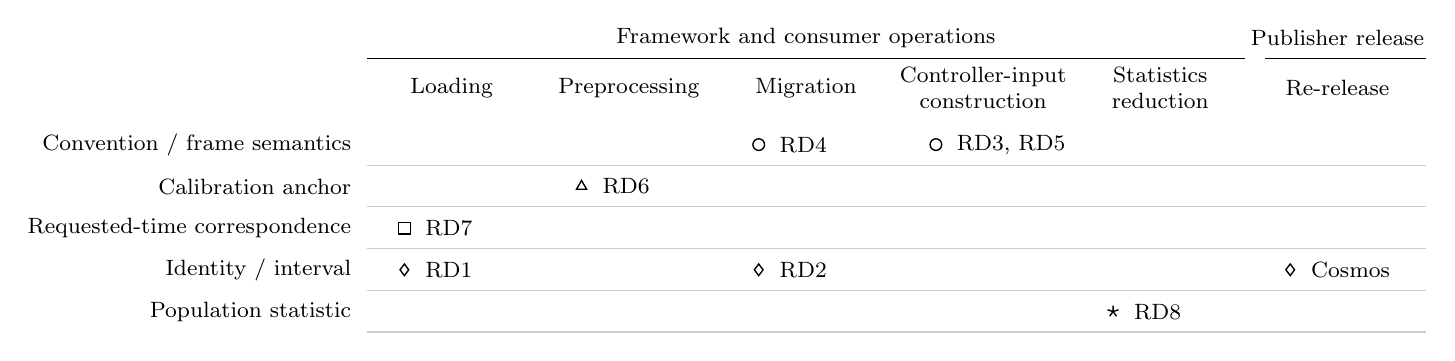
\begin{tikzpicture}[x=1cm,y=1cm,font=\rmfamily\footnotesize,inner sep=0pt]
\node[] at (8.750,0.920) {Framework and consumer operations};
\node[] at (15.500,0.920) {Publisher release};
\draw[line width=.5pt] (3.18,.65)--(14.33,.65);
\draw[line width=.5pt] (14.58,.65)--(16.63,.65);
\node[align=center] at (4.250,0.280) {Loading};
\node[align=center] at (6.500,0.280) {Preprocessing};
\node[align=center] at (8.750,0.280) {Migration};
\node[align=center] at (11.000,0.280) {Controller-input\\construction};
\node[align=center] at (13.250,0.280) {Statistics\\reduction};
\node[align=center] at (15.500,0.280) {Re-release};
\node[anchor=east] at (2.980,-0.440) {Convention / frame semantics};
\draw[black!20,line width=.4pt] (3.18,-0.700)--(16.63,-0.700);
\draw plot[mark=o,mark size=2.1pt,mark options={line width=.5pt,fill=white}] coordinates {(8.150,-0.440)};
\node[anchor=west] at (8.410,-0.440) {RD4};
\draw plot[mark=o,mark size=2.1pt,mark options={line width=.5pt,fill=white}] coordinates {(10.400,-0.440)};
\node[anchor=west] at (10.660,-0.440) {RD3, RD5};
\node[anchor=east] at (2.980,-0.970) {Calibration anchor};
\draw[black!20,line width=.4pt] (3.18,-1.230)--(16.63,-1.230);
\draw plot[mark=triangle,mark size=2.1pt,mark options={line width=.5pt,fill=white}] coordinates {(5.900,-0.970)};
\node[anchor=west] at (6.160,-0.970) {RD6};
\node[anchor=east] at (2.980,-1.500) {Requested-time correspondence};
\draw[black!20,line width=.4pt] (3.18,-1.760)--(16.63,-1.760);
\draw plot[mark=square,mark size=2.1pt,mark options={line width=.5pt,fill=white}] coordinates {(3.650,-1.500)};
\node[anchor=west] at (3.910,-1.500) {RD7};
\node[anchor=east] at (2.980,-2.030) {Identity / interval};
\draw[black!20,line width=.4pt] (3.18,-2.290)--(16.63,-2.290);
\draw plot[mark=diamond,mark size=2.1pt,mark options={line width=.5pt,fill=white}] coordinates {(3.650,-2.030)};
\node[anchor=west] at (3.910,-2.030) {RD1};
\draw plot[mark=diamond,mark size=2.1pt,mark options={line width=.5pt,fill=white}] coordinates {(8.150,-2.030)};
\node[anchor=west] at (8.410,-2.030) {RD2};
\draw plot[mark=diamond,mark size=2.1pt,mark options={line width=.5pt,fill=white}] coordinates {(14.900,-2.030)};
\node[anchor=west] at (15.160,-2.030) {Cosmos};
\node[anchor=east] at (2.980,-2.560) {Population statistic};
\draw[black!20,line width=.4pt] (3.18,-2.820)--(16.63,-2.820);
\draw plot[mark=star,mark size=2.1pt,mark options={line width=.5pt,fill=white}] coordinates {(12.650,-2.560)};
\node[anchor=west] at (12.910,-2.560) {RD8};
\end{tikzpicture}
\caption{Case coverage by operation and required semantic reference. Columns are operation categories, not a prescribed execution order; symbols distinguish reference kinds. RD3 and RD5 share a broad convention/frame-semantics category but use different rules. Cosmos is the complementary re-release audit, outside the eight-case corpus.}
\label{fig:pipeline-coverage}
\end{figure*}


The fixed release snapshot binds the original case sources to the newer validator experiment, RD8 diagnostic, Cosmos checks and figure generator in one per-file manifest \cite{13}. Each replay uses a fresh run directory, separates archived expected outcomes from newly generated results, and records executable, inputs, timing, exit status and streams. Pinned upstream downloads and bundled low-dimensional derivatives have distinct recovery and licensing entries in the registry, where full-file hashes, range-read identities and projection digests are not interchangeable.\par

Fig. 1 locates cases by operation and reference requirement. Each replay pins source and input identities, applies a fixed rule and scope, and retains its verdict, residuals, logs and environment. Paired paths receive the same inputs and unchanged complete decision rule, whereas RD4 audits one upstream converter body against its declared field inventory. Dependency, download, hash and execution failures are infrastructure outcomes; completed calculations that fail their scientific rules, such as RD8, remain separate retained results.\par

For a minimal executable reuse path, obtain the fixed snapshot \cite{13}, install its pinned dependencies and run \texttt{python run\_\allowbreak{}\allowbreak{}public.py -{}-suite gx -{}-download -{}-work-dir /\allowbreak{}tmp/\allowbreak{}rdr-new}. This creates a fresh run directory, verifies bundled projection identities, fetches hash-checked inputs, constructs seven faulty/reference fixture pairs and executes 42 native GX validations with six frozen-result comparisons. The output distinguishes expected scientific outcomes, scientific mismatches and infrastructure failures, allowing researchers to inspect the case rules, reference fixtures and raw verdicts when evaluating their own checks. These known cases are developer-visible examples, not an unseen generalization test set.\par

\subsection{Execution objects and reference authority}

\textbf{E1} denotes exact upstream before/after execution, \textbf{E2} a historical branch or loop replay, and \textbf{E3} an exact-constant or minimal-path experiment. Table I records each case's scope rather than assigning the whole resource one fidelity label. RD4 is an \textbf{upstream-body audit}, with unused imports stubbed and a NumPy-equivalent permutation helper; no repaired converter is executed. RD7 reconstructs the historical selection branches using PyAV. Source revisions and public event dates retain distinct roles: RD1 replays the proposed-fix revision, although its PR merged later \cite{2}.\par

Reference authority varies across cases. RD1 shares an expected-window helper between construction and checking, RD6 uses anchors documented by the upstream repair, and RD7's sequential reference decode uses the same decoder library as its selection branches. These dependencies are reported with the relevant outcomes rather than described as independent implementations.\par

\subsection{The eight cases}

\begin{table*}[t]
\centering
\footnotesize
\caption{Cases, local properties checked, required references and replay outcomes.}
\label{tab:cases}
\renewcommand{\arraystretch}{1.10}
\setlength{\tabcolsep}{1.5pt}
\begin{tabular}{@{}>{\raggedright\arraybackslash}p{0.58cm}>{\raggedright\arraybackslash}p{1.53cm}>{\raggedright\arraybackslash}p{1.65cm}>{\raggedright\arraybackslash}p{1.46cm}>{\raggedright\arraybackslash}p{3.2cm}>{\raggedright\arraybackslash}p{2.64cm}>{\raggedright\arraybackslash}p{5.12cm}@{}}
\toprule
\textbf{Case} & \textbf{Ecosystem} & \textbf{Stage} & \textbf{Execution} & \textbf{Local property checked} & \textbf{Required reference} & \textbf{Replay outcome} \\
\midrule
RD1 & LeRobot~\cite{2} & Loading & E3 minimal path & In-bounds index; Boolean pad & Absolute row identity & 118/118 $\rightarrow$ 0/118 padding violations \\
RD2 & LeRobot~\cite{4} & Migration & E2 loop & Nonnegative integers; end$-$start$=$length & Global continuity & 1/5 $\rightarrow$ 0/5 episode violations \\
RD3 & Isaac Lab~\cite{1} & Controller input & E3 constant & Width four; finite; unit norm & Quaternion convention & $120^{\circ} \to 0^{\circ}$ orientation error \\
RD4 & Isaac Lab~\cite{3} & Migration & Body audit & Shape; finite; format/version & Field inventory; convention & 15,141/23,833 unconverted instances \\
RD5 & robosuite~\cite{5} & Controller input & E2 branch & Raw input shape; $[-1,1]$ range & Displacement semantics & 9,666/9,666 $\rightarrow$ 0/9,666 violations \\
RD6 & OpenPI~\cite{6} & Preprocessing & E2 branch & Finite anchors; old-only round-trip & Encoder anchors & 2/2 $\rightarrow$ 0/2 anchor violations \\
RD7 & GR00T~\cite{7} & Loading & E2 branch & Count, shape, dtype; readability & Requested-time mapping & 200/200 $\rightarrow$ 0/200 wrong non-control frames \\
RD8 & OpenPI~\cite{8} & Statistics & E2 reducer & Finite mean/std; std $\geq0$ & Population statistic & \textbf{Negative:} 24/44 conditions fail \\
\bottomrule
\end{tabular}
\par\vspace{3pt}
\begin{minipage}{\textwidth}\footnotesize
Arrows: faulty $\to$ reference; denominators are case-specific. E2: branch/loop; E3: constant/minimal path. RD4 is an unpaired audit; RD5 checks raw input, not transformed displacement; RD6 round-trip applies only to the old pair. RD1 bare-index disagreement: 117/118; RD7 controls: 2,038 correct. RD8 restores 36,900/36,900 rows, but 24/44 conditions exceed $10^{-5}$ (max $ 3.235\times10^{-4}$). Exact local-check definitions and scopes are in the registry.
\end{minipage}
\end{table*}


Table I identifies each case's operation stage, execution scope, tested local property, reference requirement and outcome, while the registry supplies source revisions, local checks and complete decision rules. Two distinctions matter when interpreting the counts.\par

First, RD3 and RD4 share the same representation-convention problem but exercise different source paths and objects: a configuration constant versus migration coverage. They are distinct cases, not independent mechanism categories, and their numbers must not be merged. RD3 is one configuration constant 120\(^{\circ}\) from its intended rotation under the angular rule \(2\arccos(|q_{\mathrm{ref}}\cdot q_{\mathrm{out}}|)\), applied after normalization and convention alignment so \(q\) and \(-q\) stay equivalent. RD4's 15,141 unconverted instances are each more than 90\(^{\circ}\) away, averaging 149.17\(^{\circ}\). Second, RD1 reports two metrics: all 118 of 118 window decisions violate the padding and contract rule, while comparing only the bare returned index against the source index leaves 117 of 118 differing because one value coincides. Quoting 118 as "118 wrong indices" would therefore be wrong. RD8 is treated in Section IV-C.\par

\textbf{RD4's inventory follows the declared migration semantics.} The pinned converter labels legacy format 0 as WXYZ and format 1 as XYZW; its method documents conversion of all quaternion values and writes the new format version \cite{3}. The stack task configuration names \texttt{cube\_\allowbreak{}\allowbreak{}orientations}, \texttt{eef\_\allowbreak{}\allowbreak{}quat} and \texttt{object}, whose producer functions read cube root orientations, the end-effector frame quaternion and embedded cube-quaternion slices \cite{32}. The corresponding root and frame data definitions explicitly specify WXYZ \cite{33}, so the inventory uses named fields and producer semantics, not array width alone. Across the ten demonstrations, it covers 8,692 \texttt{root\_\allowbreak{}\allowbreak{}pose} quaternions, 6,489 \texttt{cube\_\allowbreak{}\allowbreak{}orientations} entries, 2,163 \texttt{eef\_\allowbreak{}\allowbreak{}quat} entries and 6,489 quaternion slices inside \texttt{object}. The executed converter selects only width-seven \texttt{root\_\allowbreak{}\allowbreak{}pose} arrays, converting 8,692 of 23,833 serialized instances and leaving 15,141 in WXYZ while labeling the file XYZW. The latter count includes duplicated cube representations stored in two fields, which are separate migration obligations, not independent physical samples. This is a coverage verdict under the pinned converter's stated format contract; no repaired converter or downstream replay is inferred.\par

\section{Reference Requirements and Rule Portability}

\subsection{What each replay establishes}

Across cases, Table I identifies three principal reference requirements, each demonstrated by executed checks.\par

\textbf{Finding 1: Coefficient equality does not establish physical equivalence.} RD3's faulty tuple is literally equal to its source while its correctly reordered tuple differs numerically; all 15,141 uncovered RD4 instances likewise retain their source coefficients. Checking orientation preservation therefore requires the conventions as well as the coefficients.\par

\textbf{Finding 2: Round-trip consistency does not establish calibration correctness.} RD6 provides a complete two-anchor example. The upstream repair documents encoder counts \(e\in\{2405,3110\}\), zero at 2,048 and 4,096 counts per revolution \cite{6}, giving angles \(\theta(e)=2\pi(e-2048)/4096\) and expected normalized endpoints \(y\in\{0,1\}\). The old calculation \(N_{\mathrm{old}}(\theta)=(\theta-0.4)/(1.5-0.4)\) has an exact inverse at both tested inputs, with measured round-trip errors of zero, yet yields 0.134210 and 1.117352 at those anchors. The semantic rule requires \(\max_e |N(\theta(e))-y_e|\leq 10^{-3}\). The old maximum error of 0.134210 fails this rule, whereas the repaired normalization using endpoints 0.5476 and 1.6296 yields a maximum error of 0.000474 and passes. This verdict covers the two documented anchors: internal invertibility establishes agreement between transforms, while the anchors establish their calibration.\par

\textbf{Finding 3: Frame readability does not establish requested-time correspondence.} RD7 returns correctly shaped images in both branches, yet the old branch selects the wrong frames for all 200 non-control requests. Pairing each request with its intended timestamp and frame identity exposes the error.\par

Two further requirements extend these findings. RD1 and RD2 need an \textbf{identity or interval relation}---absolute row identity and continuity of global episode intervals across output files---expressible from the artifact's own fields but not established by the row-local structural checks evaluated here. RD8 needs a \textbf{population statistic}: an independently computed full-array reference, against which coverage and numerical agreement are separate requirements. The Cosmos audit in Section V examines an identity relation of the same kind, between a summary and the frames it summarizes, with the reference inside the same release.\par

Such references can be release-internal: RD5's declared controller range separates its faulty output, and Cosmos summaries can be compared with their own collection. Across these cases, the relevant relation must be stated explicitly rather than assumed to follow from structural acceptance.\par

\subsection{Carrying the case rules into a general-purpose validator}

To test rule portability into an existing validation host, we executed the case rules natively in Great Expectations 1.6.3 on paired faulty and reference artifacts \cite{18}. The protocol, eligible cases, suites, fixtures and scoring rule were hashed before execution; failed and superseded runs remain in the release record.\par

\begin{table}[t]
\centering
\footnotesize
\caption{Per-case paired outcomes in native Great Expectations 1.6.3.}
\label{tab:gx}
\renewcommand{\arraystretch}{1.12}
\setlength{\tabcolsep}{5pt}
\begin{tabular}{@{}lcccl@{}}
\toprule
\textbf{Case} & \textbf{A} & \textbf{B} & \textbf{C} & \textbf{C: flagged / applicable} \\
\midrule
RD1 & $\circ$ & $\times$ & $\checkmark$ & 118/118 $\to$ 0/118 \\
RD2 & $\circ$ & $\times$ & $\checkmark$ & 1/5 $\to$ 0/5 \\
RD3 & \multicolumn{3}{c}{NA} & --- \\
RD4 & $\circ$ & $\times$ & $\checkmark$ & 15,141/23,833 $\to$ 0/23,833 \\
RD5 & $\checkmark$ & $\times$ & $\checkmark$ & 9,666/9,666 $\to$ 0/9,666 \\
RD6 & $\times$ & $\times$ & $\checkmark$ & 2/2 $\to$ 0/2 \\
RD7 & $\circ$ & $\times$ & $\checkmark$ & 200/2,238 $\to$ 0/2,238 \\
RD8 & $\circ$ & $\checkmark$ & $\checkmark$ & 28/28 $\to$ 0/28 \\
\midrule
Separated & 1/7 & 1/7 & 7/7 & faulty $\to$ reference \\
\bottomrule
\end{tabular}
\par\vspace{3pt}
\begin{minipage}{\columnwidth}\footnotesize
A: declared; B: reference-fitted; C: case-informed. $\checkmark$: faulty rejected/reference accepted; $\circ$: both accepted; $\times$: both rejected. RD3 is NA. RD4 uses a constructed reference; RD6 covers 2 anchors (73,800 other rows outside scope); RD7 includes controls; RD8 counts feature-statistic records at the primary condition. No reference-only rejections occurred. Predicates and references vary; counts assess supplied-rule portability.
\end{minipage}
\end{table}


Seven cases yield a columnar artifact with more than one record. RD3 is not applicable because its replay object is a single configuration constant whose defect appears at population scale as RD4. Table II reports each pair outcome, with construction scopes that differ across the seven pairings. RD1, RD2, RD5, RD7 and RD8 pair a faulty output with the repaired branch's output. RD4's reference conversion applies the declared permutation to every source tuple, because no repaired upstream converter is executed in this study. RD6 uses a derived target whose anchor predicate constrains only the two calibration anchor rows of a 73,802-row batch; the remaining rows are outside its scope, and its frozen replay unit is unchanged. RD8's artifact is the archived primary condition alone, natural order at batch 32, chosen before these runs; it says nothing about the other 43 conditions.\par

The suites differ in both the available reference information \textit{and} the predicates consuming it, while framework, executor, versions and scoring remain identical. \textbf{Declared} uses structure and range expectations justified by each artifact's declared schema and documentation. \textbf{Reference-fitted} applies one mechanical rule---column set, non-null, dtype, observed minimum and maximum, observed value set for low-cardinality columns---to a reference fixture. For six cases, this fixture is a disjoint split of the reference artifact by row, demonstration or video. RD8's 28 component records (14 state and 14 action dimensions) admit no exchangeable split, so its fixture is the separately published companion statistics table, a distinct artifact whose population may overlap the evaluated projection. \textbf{Case-informed} supplies the case's own reference information through Expectation classes registered into the framework. A pair is separated only when the faulty artifact is rejected \textit{and} the paired reference artifact is accepted.\par

The declared suite separates one pair of seven: RD5. Its controller declares a per-axis output range of ±0.05 m, so with this fixture's identity base rotation the displacement-norm bound is \(\sqrt{3}\times 0.05 = 0.0866\) m. Three expectations reject all 9,666 faulty rows, whose norm reaches 1.127 m, while accepting the repaired artifact at 0.072 m; this expected separation was recorded before execution. On RD6, however, the suite rejects \textit{both} artifacts because real gripper values leave the documented 0--1 range under both normalizations. The reference-fitted suite separates only RD8, using the companion fixture above. It rejects both paired artifacts in the other six cases because bounds fitted on one disjoint split also fail to cover the held-out split. This result concerns these seven artifacts under one mechanical rule, not profiling systems in general.\par

The case-informed suite rejects all seven faulty artifacts at exactly the counts reported in the case records and accepts all seven reference artifacts. Clamp-and-pad row identity, global interval chaining, quaternion convention, displacement versus position, calibration anchors, requested-time correspondence and agreement with an independent reference statistic are all expressible as Expectation classes, each separating its tested pair. This establishes a bounded portability result: the corpus's rules and reference artifacts port to a general-purpose validation tool and separate faulty from reference outputs there. Because predicates and reference data vary together, the experiment measures neither automatic discovery accuracy nor the causal value of reference information.\par

These outcomes ground the three findings in executed checks. The declared suite accepts all 23,833 RD4 quaternions---including the 15,141 retaining their source coefficients---while the convention-aware expectation rejects exactly those. It cannot separate the two RD6 branches, whereas the anchor expectation rejects both faulty anchors and accepts both reference ones. It also accepts all 2,238 RD7 responses as correctly shaped \texttt{uint8} images in both branches, while the correspondence expectation rejects exactly the 200 non-control requests.\par

\subsection{The negative case, kept complete}

RD8 replays a reducer that computes normalization statistics from only the first member of each batch \cite{8}. Its frozen input comprises all 123 episodes and 36,900 rows of a pinned ALOHA dataset, projected to 14-component state and action vectors plus episode, frame and timestamp columns. The runner preserves natural order plus ten complete episode-cluster orders, seeds 0--9, across batch sizes 1, 8, 32 and 128: 44 conditions, including every nonempty final partial batch. It deliberately differs from the historical loader's separate \texttt{drop\_\allowbreak{}\allowbreak{}last=True} behavior and omits its action horizon, ALOHA transforms and image-bearing DataLoader to isolate the raw-feature reducer branch. An independently computed float64 full-array reference supplies count, mean, population standard deviation and percentiles. Fixed means and standard deviations must meet absolute tolerance \(10^{-5}\) in every condition; quantiles remain descriptive because the historical reducer uses an approximate histogram.\par

\begin{figure}[t]
\centering
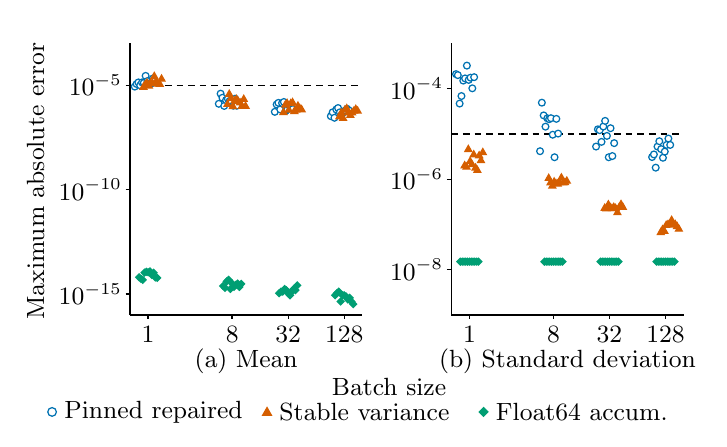
\begin{tikzpicture}[x=1cm,y=1cm,font=\rmfamily\fontsize{9}{10.5}\selectfont,inner sep=0pt,text=black]
\definecolor{rdPinned}{HTML}{0072B2}
\definecolor{rdStable}{HTML}{D55E00}
\definecolor{rdAccum}{HTML}{009E73}
\path[use as bounding box] (0,-1.32) rectangle (8.52,3.65);
\draw[line width=0.5pt] (1.30000,0) -- (4.25000,0);
\draw[line width=0.5pt] (1.30000,0) -- (1.30000,3.45000);
\draw[line width=0.5pt] (1.24500,0.26538) -- (1.30000,0.26538);
\node[anchor=east] at (1.20500,0.26538) {$10^{-15}$};
\draw[line width=0.5pt] (1.24500,1.59231) -- (1.30000,1.59231);
\node[anchor=east] at (1.20500,1.59231) {$10^{-10}$};
\draw[line width=0.5pt] (1.24500,2.91923) -- (1.30000,2.91923);
\node[anchor=east] at (1.20500,2.91923) {$10^{-5}$};
\draw[line width=0.5pt] (1.53000,0) -- (1.53000,-0.055);
\node[anchor=north] at (1.53000,-0.14000) {1};
\draw[line width=0.5pt] (2.59714,0) -- (2.59714,-0.055);
\node[anchor=north] at (2.59714,-0.14000) {8};
\draw[line width=0.5pt] (3.30857,0) -- (3.30857,-0.055);
\node[anchor=north] at (3.30857,-0.14000) {32};
\draw[line width=0.5pt] (4.02000,0) -- (4.02000,-0.055);
\node[anchor=north] at (4.02000,-0.14000) {128};
\draw[black,line width=0.5pt,dash pattern=on 2.4pt off 1.8pt] (1.30000,2.91923) -- (4.25000,2.91923);
\draw[draw=rdPinned,fill=white,line width=0.45pt] (1.36000,2.90126) circle[radius=0.04300cm];
\draw[draw=rdPinned,fill=white,line width=0.45pt] (2.42714,2.68300) circle[radius=0.04300cm];
\draw[draw=rdPinned,fill=white,line width=0.45pt] (3.13857,2.58101) circle[radius=0.04300cm];
\draw[draw=rdPinned,fill=white,line width=0.45pt] (3.85000,2.52636) circle[radius=0.04300cm];
\draw[draw=rdPinned,fill=white,line width=0.45pt] (1.38300,2.93507) circle[radius=0.04300cm];
\draw[draw=rdPinned,fill=white,line width=0.45pt] (2.45014,2.81184) circle[radius=0.04300cm];
\draw[draw=rdPinned,fill=white,line width=0.45pt] (3.16157,2.67454) circle[radius=0.04300cm];
\draw[draw=rdPinned,fill=white,line width=0.45pt] (3.87300,2.57502) circle[radius=0.04300cm];
\draw[draw=rdPinned,fill=white,line width=0.45pt] (1.40600,2.95484) circle[radius=0.04300cm];
\draw[draw=rdPinned,fill=white,line width=0.45pt] (2.47314,2.75982) circle[radius=0.04300cm];
\draw[draw=rdPinned,fill=white,line width=0.45pt] (3.18457,2.69548) circle[radius=0.04300cm];
\draw[draw=rdPinned,fill=white,line width=0.45pt] (3.89600,2.50567) circle[radius=0.04300cm];
\draw[draw=rdPinned,fill=white,line width=0.45pt] (1.42900,2.91706) circle[radius=0.04300cm];
\draw[draw=rdPinned,fill=white,line width=0.45pt] (2.49614,2.65592) circle[radius=0.04300cm];
\draw[draw=rdPinned,fill=white,line width=0.45pt] (3.20757,2.61130) circle[radius=0.04300cm];
\draw[draw=rdPinned,fill=white,line width=0.45pt] (3.91900,2.61082) circle[radius=0.04300cm];
\draw[draw=rdPinned,fill=white,line width=0.45pt] (1.45200,2.95486) circle[radius=0.04300cm];
\draw[draw=rdPinned,fill=white,line width=0.45pt] (2.51914,2.72988) circle[radius=0.04300cm];
\draw[draw=rdPinned,fill=white,line width=0.45pt] (3.23057,2.69293) circle[radius=0.04300cm];
\draw[draw=rdPinned,fill=white,line width=0.45pt] (3.94200,2.62923) circle[radius=0.04300cm];
\draw[draw=rdPinned,fill=white,line width=0.45pt] (1.47500,2.94937) circle[radius=0.04300cm];
\draw[draw=rdPinned,fill=white,line width=0.45pt] (2.54214,2.74670) circle[radius=0.04300cm];
\draw[draw=rdPinned,fill=white,line width=0.45pt] (3.25357,2.70631) circle[radius=0.04300cm];
\draw[draw=rdPinned,fill=white,line width=0.45pt] (3.96500,2.57479) circle[radius=0.04300cm];
\draw[draw=rdPinned,fill=white,line width=0.45pt] (1.49800,3.03807) circle[radius=0.04300cm];
\draw[draw=rdPinned,fill=white,line width=0.45pt] (2.56514,2.71909) circle[radius=0.04300cm];
\draw[draw=rdPinned,fill=white,line width=0.45pt] (3.27657,2.59333) circle[radius=0.04300cm];
\draw[draw=rdPinned,fill=white,line width=0.45pt] (3.98800,2.54366) circle[radius=0.04300cm];
\draw[draw=rdPinned,fill=white,line width=0.45pt] (1.52100,2.97216) circle[radius=0.04300cm];
\draw[draw=rdPinned,fill=white,line width=0.45pt] (2.58814,2.70254) circle[radius=0.04300cm];
\draw[draw=rdPinned,fill=white,line width=0.45pt] (3.29957,2.61138) circle[radius=0.04300cm];
\draw[draw=rdPinned,fill=white,line width=0.45pt] (4.01100,2.57479) circle[radius=0.04300cm];
\draw[draw=rdPinned,fill=white,line width=0.45pt] (1.54400,2.94181) circle[radius=0.04300cm];
\draw[draw=rdPinned,fill=white,line width=0.45pt] (2.61114,2.65904) circle[radius=0.04300cm];
\draw[draw=rdPinned,fill=white,line width=0.45pt] (3.32257,2.66147) circle[radius=0.04300cm];
\draw[draw=rdPinned,fill=white,line width=0.45pt] (4.03400,2.59928) circle[radius=0.04300cm];
\draw[draw=rdPinned,fill=white,line width=0.45pt] (1.56700,2.93944) circle[radius=0.04300cm];
\draw[draw=rdPinned,fill=white,line width=0.45pt] (2.63414,2.74784) circle[radius=0.04300cm];
\draw[draw=rdPinned,fill=white,line width=0.45pt] (3.34557,2.62997) circle[radius=0.04300cm];
\draw[draw=rdPinned,fill=white,line width=0.45pt] (4.05700,2.61946) circle[radius=0.04300cm];
\draw[draw=rdPinned,fill=white,line width=0.45pt] (1.59000,3.00478) circle[radius=0.04300cm];
\draw[draw=rdPinned,fill=white,line width=0.45pt] (2.65714,2.65880) circle[radius=0.04300cm];
\draw[draw=rdPinned,fill=white,line width=0.45pt] (3.36857,2.61595) circle[radius=0.04300cm];
\draw[draw=rdPinned,fill=white,line width=0.45pt] (4.08000,2.59928) circle[radius=0.04300cm];
\path[draw=rdStable,fill=rdStable,line width=0.45pt] (1.47000,2.94426) -- (1.42700,2.86901) -- (1.51300,2.86901) -- cycle;
\path[draw=rdStable,fill=rdStable,line width=0.45pt] (2.53714,2.72600) -- (2.49414,2.65075) -- (2.58014,2.65075) -- cycle;
\path[draw=rdStable,fill=rdStable,line width=0.45pt] (3.24857,2.62401) -- (3.20557,2.54876) -- (3.29157,2.54876) -- cycle;
\path[draw=rdStable,fill=rdStable,line width=0.45pt] (3.96000,2.56936) -- (3.91700,2.49411) -- (4.00300,2.49411) -- cycle;
\path[draw=rdStable,fill=rdStable,line width=0.45pt] (1.49300,2.97807) -- (1.45000,2.90282) -- (1.53600,2.90282) -- cycle;
\path[draw=rdStable,fill=rdStable,line width=0.45pt] (2.56014,2.85484) -- (2.51714,2.77959) -- (2.60314,2.77959) -- cycle;
\path[draw=rdStable,fill=rdStable,line width=0.45pt] (3.27157,2.71754) -- (3.22857,2.64229) -- (3.31457,2.64229) -- cycle;
\path[draw=rdStable,fill=rdStable,line width=0.45pt] (3.98300,2.61802) -- (3.94000,2.54277) -- (4.02600,2.54277) -- cycle;
\path[draw=rdStable,fill=rdStable,line width=0.45pt] (1.51600,2.99784) -- (1.47300,2.92259) -- (1.55900,2.92259) -- cycle;
\path[draw=rdStable,fill=rdStable,line width=0.45pt] (2.58314,2.80282) -- (2.54014,2.72757) -- (2.62614,2.72757) -- cycle;
\path[draw=rdStable,fill=rdStable,line width=0.45pt] (3.29457,2.73848) -- (3.25157,2.66323) -- (3.33757,2.66323) -- cycle;
\path[draw=rdStable,fill=rdStable,line width=0.45pt] (4.00600,2.54867) -- (3.96300,2.47342) -- (4.04900,2.47342) -- cycle;
\path[draw=rdStable,fill=rdStable,line width=0.45pt] (1.53900,2.96006) -- (1.49600,2.88481) -- (1.58200,2.88481) -- cycle;
\path[draw=rdStable,fill=rdStable,line width=0.45pt] (2.60614,2.69892) -- (2.56314,2.62367) -- (2.64914,2.62367) -- cycle;
\path[draw=rdStable,fill=rdStable,line width=0.45pt] (3.31757,2.65430) -- (3.27457,2.57905) -- (3.36057,2.57905) -- cycle;
\path[draw=rdStable,fill=rdStable,line width=0.45pt] (4.02900,2.65382) -- (3.98600,2.57857) -- (4.07200,2.57857) -- cycle;
\path[draw=rdStable,fill=rdStable,line width=0.45pt] (1.56200,2.99786) -- (1.51900,2.92261) -- (1.60500,2.92261) -- cycle;
\path[draw=rdStable,fill=rdStable,line width=0.45pt] (2.62914,2.77288) -- (2.58614,2.69763) -- (2.67214,2.69763) -- cycle;
\path[draw=rdStable,fill=rdStable,line width=0.45pt] (3.34057,2.73593) -- (3.29757,2.66068) -- (3.38357,2.66068) -- cycle;
\path[draw=rdStable,fill=rdStable,line width=0.45pt] (4.05200,2.67223) -- (4.00900,2.59698) -- (4.09500,2.59698) -- cycle;
\path[draw=rdStable,fill=rdStable,line width=0.45pt] (1.58500,2.99237) -- (1.54200,2.91712) -- (1.62800,2.91712) -- cycle;
\path[draw=rdStable,fill=rdStable,line width=0.45pt] (2.65214,2.78970) -- (2.60914,2.71445) -- (2.69514,2.71445) -- cycle;
\path[draw=rdStable,fill=rdStable,line width=0.45pt] (3.36357,2.74931) -- (3.32057,2.67406) -- (3.40657,2.67406) -- cycle;
\path[draw=rdStable,fill=rdStable,line width=0.45pt] (4.07500,2.61779) -- (4.03200,2.54254) -- (4.11800,2.54254) -- cycle;
\path[draw=rdStable,fill=rdStable,line width=0.45pt] (1.60800,3.08107) -- (1.56500,3.00582) -- (1.65100,3.00582) -- cycle;
\path[draw=rdStable,fill=rdStable,line width=0.45pt] (2.67514,2.76209) -- (2.63214,2.68684) -- (2.71814,2.68684) -- cycle;
\path[draw=rdStable,fill=rdStable,line width=0.45pt] (3.38657,2.63633) -- (3.34357,2.56108) -- (3.42957,2.56108) -- cycle;
\path[draw=rdStable,fill=rdStable,line width=0.45pt] (4.09800,2.58666) -- (4.05500,2.51141) -- (4.14100,2.51141) -- cycle;
\path[draw=rdStable,fill=rdStable,line width=0.45pt] (1.63100,3.01516) -- (1.58800,2.93991) -- (1.67400,2.93991) -- cycle;
\path[draw=rdStable,fill=rdStable,line width=0.45pt] (2.69814,2.74554) -- (2.65514,2.67029) -- (2.74114,2.67029) -- cycle;
\path[draw=rdStable,fill=rdStable,line width=0.45pt] (3.40957,2.65438) -- (3.36657,2.57913) -- (3.45257,2.57913) -- cycle;
\path[draw=rdStable,fill=rdStable,line width=0.45pt] (4.12100,2.61779) -- (4.07800,2.54254) -- (4.16400,2.54254) -- cycle;
\path[draw=rdStable,fill=rdStable,line width=0.45pt] (1.65400,2.98481) -- (1.61100,2.90956) -- (1.69700,2.90956) -- cycle;
\path[draw=rdStable,fill=rdStable,line width=0.45pt] (2.72114,2.70204) -- (2.67814,2.62679) -- (2.76414,2.62679) -- cycle;
\path[draw=rdStable,fill=rdStable,line width=0.45pt] (3.43257,2.70447) -- (3.38957,2.62922) -- (3.47557,2.62922) -- cycle;
\path[draw=rdStable,fill=rdStable,line width=0.45pt] (4.14400,2.64228) -- (4.10100,2.56703) -- (4.18700,2.56703) -- cycle;
\path[draw=rdStable,fill=rdStable,line width=0.45pt] (1.67700,2.98244) -- (1.63400,2.90719) -- (1.72000,2.90719) -- cycle;
\path[draw=rdStable,fill=rdStable,line width=0.45pt] (2.74414,2.79084) -- (2.70114,2.71559) -- (2.78714,2.71559) -- cycle;
\path[draw=rdStable,fill=rdStable,line width=0.45pt] (3.45557,2.67297) -- (3.41257,2.59772) -- (3.49857,2.59772) -- cycle;
\path[draw=rdStable,fill=rdStable,line width=0.45pt] (4.16700,2.66246) -- (4.12400,2.58721) -- (4.21000,2.58721) -- cycle;
\path[draw=rdStable,fill=rdStable,line width=0.45pt] (1.70000,3.04778) -- (1.65700,2.97253) -- (1.74300,2.97253) -- cycle;
\path[draw=rdStable,fill=rdStable,line width=0.45pt] (2.76714,2.70180) -- (2.72414,2.62655) -- (2.81014,2.62655) -- cycle;
\path[draw=rdStable,fill=rdStable,line width=0.45pt] (3.47857,2.65895) -- (3.43557,2.58370) -- (3.52157,2.58370) -- cycle;
\path[draw=rdStable,fill=rdStable,line width=0.45pt] (4.19000,2.64228) -- (4.14700,2.56703) -- (4.23300,2.56703) -- cycle;
\path[draw=rdAccum,fill=rdAccum,line width=0.45pt] (1.41500,0.52304) -- (1.45800,0.48004) -- (1.41500,0.43704) -- (1.37200,0.48004) -- cycle;
\path[draw=rdAccum,fill=rdAccum,line width=0.45pt] (2.48214,0.41131) -- (2.52514,0.36831) -- (2.48214,0.32531) -- (2.43914,0.36831) -- cycle;
\path[draw=rdAccum,fill=rdAccum,line width=0.45pt] (3.19357,0.32044) -- (3.23657,0.27744) -- (3.19357,0.23444) -- (3.15057,0.27744) -- cycle;
\path[draw=rdAccum,fill=rdAccum,line width=0.45pt] (3.90500,0.29472) -- (3.94800,0.25172) -- (3.90500,0.20872) -- (3.86200,0.25172) -- cycle;
\path[draw=rdAccum,fill=rdAccum,line width=0.45pt] (1.43800,0.50360) -- (1.48100,0.46060) -- (1.43800,0.41760) -- (1.39500,0.46060) -- cycle;
\path[draw=rdAccum,fill=rdAccum,line width=0.45pt] (2.50514,0.38818) -- (2.54814,0.34518) -- (2.50514,0.30218) -- (2.46214,0.34518) -- cycle;
\path[draw=rdAccum,fill=rdAccum,line width=0.45pt] (3.21657,0.34145) -- (3.25957,0.29845) -- (3.21657,0.25545) -- (3.17357,0.29845) -- cycle;
\path[draw=rdAccum,fill=rdAccum,line width=0.45pt] (3.92800,0.32044) -- (3.97100,0.27744) -- (3.92800,0.23444) -- (3.88500,0.27744) -- cycle;
\path[draw=rdAccum,fill=rdAccum,line width=0.45pt] (1.46100,0.49120) -- (1.50400,0.44820) -- (1.46100,0.40520) -- (1.41800,0.44820) -- cycle;
\path[draw=rdAccum,fill=rdAccum,line width=0.45pt] (2.52814,0.47123) -- (2.57114,0.42823) -- (2.52814,0.38523) -- (2.48514,0.42823) -- cycle;
\path[draw=rdAccum,fill=rdAccum,line width=0.45pt] (3.23957,0.34145) -- (3.28257,0.29845) -- (3.23957,0.25545) -- (3.19657,0.29845) -- cycle;
\path[draw=rdAccum,fill=rdAccum,line width=0.45pt] (3.95100,0.34145) -- (3.99400,0.29845) -- (3.95100,0.25545) -- (3.90800,0.29845) -- cycle;
\path[draw=rdAccum,fill=rdAccum,line width=0.45pt] (1.48400,0.58112) -- (1.52700,0.53812) -- (1.48400,0.49512) -- (1.44100,0.53812) -- cycle;
\path[draw=rdAccum,fill=rdAccum,line width=0.45pt] (2.55114,0.49120) -- (2.59414,0.44820) -- (2.55114,0.40520) -- (2.50814,0.44820) -- cycle;
\path[draw=rdAccum,fill=rdAccum,line width=0.45pt] (3.26257,0.37461) -- (3.30557,0.33161) -- (3.26257,0.28861) -- (3.21957,0.33161) -- cycle;
\path[draw=rdAccum,fill=rdAccum,line width=0.45pt] (3.97400,0.21483) -- (4.01700,0.17183) -- (3.97400,0.12883) -- (3.93100,0.17183) -- cycle;
\path[draw=rdAccum,fill=rdAccum,line width=0.45pt] (1.50700,0.59254) -- (1.55000,0.54954) -- (1.50700,0.50654) -- (1.46400,0.54954) -- cycle;
\path[draw=rdAccum,fill=rdAccum,line width=0.45pt] (2.57414,0.37461) -- (2.61714,0.33161) -- (2.57414,0.28861) -- (2.53114,0.33161) -- cycle;
\path[draw=rdAccum,fill=rdAccum,line width=0.45pt] (3.28557,0.35922) -- (3.32857,0.31622) -- (3.28557,0.27322) -- (3.24257,0.31622) -- cycle;
\path[draw=rdAccum,fill=rdAccum,line width=0.45pt] (3.99700,0.29472) -- (4.04000,0.25172) -- (3.99700,0.20872) -- (3.95400,0.25172) -- cycle;
\path[draw=rdAccum,fill=rdAccum,line width=0.45pt] (1.53000,0.58582) -- (1.57300,0.54282) -- (1.53000,0.49982) -- (1.48700,0.54282) -- cycle;
\path[draw=rdAccum,fill=rdAccum,line width=0.45pt] (2.59714,0.44315) -- (2.64014,0.40015) -- (2.59714,0.35715) -- (2.55414,0.40015) -- cycle;
\path[draw=rdAccum,fill=rdAccum,line width=0.45pt] (3.30857,0.32044) -- (3.35157,0.27744) -- (3.30857,0.23444) -- (3.26557,0.27744) -- cycle;
\path[draw=rdAccum,fill=rdAccum,line width=0.45pt] (4.02000,0.29472) -- (4.06300,0.25172) -- (4.02000,0.20872) -- (3.97700,0.25172) -- cycle;
\path[draw=rdAccum,fill=rdAccum,line width=0.45pt] (1.55300,0.59681) -- (1.59600,0.55381) -- (1.55300,0.51081) -- (1.51000,0.55381) -- cycle;
\path[draw=rdAccum,fill=rdAccum,line width=0.45pt] (2.62014,0.40032) -- (2.66314,0.35732) -- (2.62014,0.31432) -- (2.57714,0.35732) -- cycle;
\path[draw=rdAccum,fill=rdAccum,line width=0.45pt] (3.33157,0.29472) -- (3.37457,0.25172) -- (3.33157,0.20872) -- (3.28857,0.25172) -- cycle;
\path[draw=rdAccum,fill=rdAccum,line width=0.45pt] (4.04300,0.27933) -- (4.08600,0.23633) -- (4.04300,0.19333) -- (4.00000,0.23633) -- cycle;
\path[draw=rdAccum,fill=rdAccum,line width=0.45pt] (1.57600,0.55419) -- (1.61900,0.51119) -- (1.57600,0.46819) -- (1.53300,0.51119) -- cycle;
\path[draw=rdAccum,fill=rdAccum,line width=0.45pt] (2.64314,0.42604) -- (2.68614,0.38304) -- (2.64314,0.34004) -- (2.60014,0.38304) -- cycle;
\path[draw=rdAccum,fill=rdAccum,line width=0.45pt] (3.35457,0.34145) -- (3.39757,0.29845) -- (3.35457,0.25545) -- (3.31157,0.29845) -- cycle;
\path[draw=rdAccum,fill=rdAccum,line width=0.45pt] (4.06600,0.24055) -- (4.10900,0.19755) -- (4.06600,0.15455) -- (4.02300,0.19755) -- cycle;
\path[draw=rdAccum,fill=rdAccum,line width=0.45pt] (1.59900,0.58112) -- (1.64200,0.53812) -- (1.59900,0.49512) -- (1.55600,0.53812) -- cycle;
\path[draw=rdAccum,fill=rdAccum,line width=0.45pt] (2.66614,0.44315) -- (2.70914,0.40015) -- (2.66614,0.35715) -- (2.62314,0.40015) -- cycle;
\path[draw=rdAccum,fill=rdAccum,line width=0.45pt] (3.37757,0.37461) -- (3.42057,0.33161) -- (3.37757,0.28861) -- (3.33457,0.33161) -- cycle;
\path[draw=rdAccum,fill=rdAccum,line width=0.45pt] (4.08900,0.26156) -- (4.13200,0.21856) -- (4.08900,0.17556) -- (4.04600,0.21856) -- cycle;
\path[draw=rdAccum,fill=rdAccum,line width=0.45pt] (1.62200,0.52103) -- (1.66500,0.47803) -- (1.62200,0.43503) -- (1.57900,0.47803) -- cycle;
\path[draw=rdAccum,fill=rdAccum,line width=0.45pt] (2.68914,0.40032) -- (2.73214,0.35732) -- (2.68914,0.31432) -- (2.64614,0.35732) -- cycle;
\path[draw=rdAccum,fill=rdAccum,line width=0.45pt] (3.40057,0.35922) -- (3.44357,0.31622) -- (3.40057,0.27322) -- (3.35757,0.31622) -- cycle;
\path[draw=rdAccum,fill=rdAccum,line width=0.45pt] (4.11200,0.21483) -- (4.15500,0.17183) -- (4.11200,0.12883) -- (4.06900,0.17183) -- cycle;
\path[draw=rdAccum,fill=rdAccum,line width=0.45pt] (1.64500,0.51480) -- (1.68800,0.47180) -- (1.64500,0.42880) -- (1.60200,0.47180) -- cycle;
\path[draw=rdAccum,fill=rdAccum,line width=0.45pt] (2.71214,0.43910) -- (2.75514,0.39610) -- (2.71214,0.35310) -- (2.66914,0.39610) -- cycle;
\path[draw=rdAccum,fill=rdAccum,line width=0.45pt] (3.42357,0.42134) -- (3.46657,0.37834) -- (3.42357,0.33534) -- (3.38057,0.37834) -- cycle;
\path[draw=rdAccum,fill=rdAccum,line width=0.45pt] (4.13500,0.18167) -- (4.17800,0.13867) -- (4.13500,0.09567) -- (4.09200,0.13867) -- cycle;
\node[anchor=north] at (2.77500,-0.42000) {(a) Mean};
\draw[line width=0.5pt] (5.38000,0) -- (8.33000,0);
\draw[line width=0.5pt] (5.38000,0) -- (5.38000,3.45000);
\draw[line width=0.5pt] (5.32500,0.57500) -- (5.38000,0.57500);
\node[anchor=east] at (5.28500,0.57500) {$10^{-8}$};
\draw[line width=0.5pt] (5.32500,1.72500) -- (5.38000,1.72500);
\node[anchor=east] at (5.28500,1.72500) {$10^{-6}$};
\draw[line width=0.5pt] (5.32500,2.87500) -- (5.38000,2.87500);
\node[anchor=east] at (5.28500,2.87500) {$10^{-4}$};
\draw[line width=0.5pt] (5.61000,0) -- (5.61000,-0.055);
\node[anchor=north] at (5.61000,-0.14000) {1};
\draw[line width=0.5pt] (6.67714,0) -- (6.67714,-0.055);
\node[anchor=north] at (6.67714,-0.14000) {8};
\draw[line width=0.5pt] (7.38857,0) -- (7.38857,-0.055);
\node[anchor=north] at (7.38857,-0.14000) {32};
\draw[line width=0.5pt] (8.10000,0) -- (8.10000,-0.055);
\node[anchor=north] at (8.10000,-0.14000) {128};
\draw[black,line width=0.5pt,dash pattern=on 2.4pt off 1.8pt] (5.38000,2.30000) -- (8.33000,2.30000);
\draw[draw=rdPinned,fill=white,line width=0.45pt] (5.44000,3.06016) circle[radius=0.04300cm];
\draw[draw=rdPinned,fill=white,line width=0.45pt] (6.50714,2.08119) circle[radius=0.04300cm];
\draw[draw=rdPinned,fill=white,line width=0.45pt] (7.21857,2.13999) circle[radius=0.04300cm];
\draw[draw=rdPinned,fill=white,line width=0.45pt] (7.93000,2.00699) circle[radius=0.04300cm];
\draw[draw=rdPinned,fill=white,line width=0.45pt] (5.46300,3.04752) circle[radius=0.04300cm];
\draw[draw=rdPinned,fill=white,line width=0.45pt] (6.53014,2.69736) circle[radius=0.04300cm];
\draw[draw=rdPinned,fill=white,line width=0.45pt] (7.24157,2.35914) circle[radius=0.04300cm];
\draw[draw=rdPinned,fill=white,line width=0.45pt] (7.95300,2.04017) circle[radius=0.04300cm];
\draw[draw=rdPinned,fill=white,line width=0.45pt] (5.48600,2.68604) circle[radius=0.04300cm];
\draw[draw=rdPinned,fill=white,line width=0.45pt] (6.55314,2.53589) circle[radius=0.04300cm];
\draw[draw=rdPinned,fill=white,line width=0.45pt] (7.26457,2.34818) circle[radius=0.04300cm];
\draw[draw=rdPinned,fill=white,line width=0.45pt] (7.97600,1.87203) circle[radius=0.04300cm];
\draw[draw=rdPinned,fill=white,line width=0.45pt] (5.50900,2.78178) circle[radius=0.04300cm];
\draw[draw=rdPinned,fill=white,line width=0.45pt] (6.57614,2.39292) circle[radius=0.04300cm];
\draw[draw=rdPinned,fill=white,line width=0.45pt] (7.28757,2.19960) circle[radius=0.04300cm];
\draw[draw=rdPinned,fill=white,line width=0.45pt] (7.99900,2.13987) circle[radius=0.04300cm];
\draw[draw=rdPinned,fill=white,line width=0.45pt] (5.53200,2.97764) circle[radius=0.04300cm];
\draw[draw=rdPinned,fill=white,line width=0.45pt] (6.59914,2.49928) circle[radius=0.04300cm];
\draw[draw=rdPinned,fill=white,line width=0.45pt] (7.31057,2.39466) circle[radius=0.04300cm];
\draw[draw=rdPinned,fill=white,line width=0.45pt] (8.02200,2.20780) circle[radius=0.04300cm];
\draw[draw=rdPinned,fill=white,line width=0.45pt] (5.55500,3.00566) circle[radius=0.04300cm];
\draw[draw=rdPinned,fill=white,line width=0.45pt] (6.62214,2.48768) circle[radius=0.04300cm];
\draw[draw=rdPinned,fill=white,line width=0.45pt] (7.33357,2.46638) circle[radius=0.04300cm];
\draw[draw=rdPinned,fill=white,line width=0.45pt] (8.04500,2.10761) circle[radius=0.04300cm];
\draw[draw=rdPinned,fill=white,line width=0.45pt] (5.57800,3.16814) circle[radius=0.04300cm];
\draw[draw=rdPinned,fill=white,line width=0.45pt] (6.64514,2.50026) circle[radius=0.04300cm];
\draw[draw=rdPinned,fill=white,line width=0.45pt] (7.35657,2.27579) circle[radius=0.04300cm];
\draw[draw=rdPinned,fill=white,line width=0.45pt] (8.06800,1.99780) circle[radius=0.04300cm];
\draw[draw=rdPinned,fill=white,line width=0.45pt] (5.60100,2.98685) circle[radius=0.04300cm];
\draw[draw=rdPinned,fill=white,line width=0.45pt] (6.66814,2.29033) circle[radius=0.04300cm];
\draw[draw=rdPinned,fill=white,line width=0.45pt] (7.37957,2.00436) circle[radius=0.04300cm];
\draw[draw=rdPinned,fill=white,line width=0.45pt] (8.09100,2.07593) circle[radius=0.04300cm];
\draw[draw=rdPinned,fill=white,line width=0.45pt] (5.62400,3.01522) circle[radius=0.04300cm];
\draw[draw=rdPinned,fill=white,line width=0.45pt] (6.69114,2.00436) circle[radius=0.04300cm];
\draw[draw=rdPinned,fill=white,line width=0.45pt] (7.40257,2.37345) circle[radius=0.04300cm];
\draw[draw=rdPinned,fill=white,line width=0.45pt] (8.11400,2.16097) circle[radius=0.04300cm];
\draw[draw=rdPinned,fill=white,line width=0.45pt] (5.64700,2.87989) circle[radius=0.04300cm];
\draw[draw=rdPinned,fill=white,line width=0.45pt] (6.71414,2.49197) circle[radius=0.04300cm];
\draw[draw=rdPinned,fill=white,line width=0.45pt] (7.42557,2.01957) circle[radius=0.04300cm];
\draw[draw=rdPinned,fill=white,line width=0.45pt] (8.13700,2.24204) circle[radius=0.04300cm];
\draw[draw=rdPinned,fill=white,line width=0.45pt] (5.67000,3.02150) circle[radius=0.04300cm];
\draw[draw=rdPinned,fill=white,line width=0.45pt] (6.73714,2.30509) circle[radius=0.04300cm];
\draw[draw=rdPinned,fill=white,line width=0.45pt] (7.44857,2.18361) circle[radius=0.04300cm];
\draw[draw=rdPinned,fill=white,line width=0.45pt] (8.16000,2.16097) circle[radius=0.04300cm];
\path[draw=rdStable,fill=rdStable,line width=0.45pt] (5.55000,1.94770) -- (5.50700,1.87245) -- (5.59300,1.87245) -- cycle;
\path[draw=rdStable,fill=rdStable,line width=0.45pt] (6.61714,1.78650) -- (6.57414,1.71125) -- (6.66014,1.71125) -- cycle;
\path[draw=rdStable,fill=rdStable,line width=0.45pt] (7.32857,1.40708) -- (7.28557,1.33183) -- (7.37157,1.33183) -- cycle;
\path[draw=rdStable,fill=rdStable,line width=0.45pt] (8.04000,1.09790) -- (7.99700,1.02265) -- (8.08300,1.02265) -- cycle;
\path[draw=rdStable,fill=rdStable,line width=0.45pt] (5.57300,1.92938) -- (5.53000,1.85413) -- (5.61600,1.85413) -- cycle;
\path[draw=rdStable,fill=rdStable,line width=0.45pt] (6.64014,1.73078) -- (6.59714,1.65553) -- (6.68314,1.65553) -- cycle;
\path[draw=rdStable,fill=rdStable,line width=0.45pt] (7.35157,1.39902) -- (7.30857,1.32377) -- (7.39457,1.32377) -- cycle;
\path[draw=rdStable,fill=rdStable,line width=0.45pt] (8.06300,1.13471) -- (8.02000,1.05946) -- (8.10600,1.05946) -- cycle;
\path[draw=rdStable,fill=rdStable,line width=0.45pt] (5.59600,2.15385) -- (5.55300,2.07860) -- (5.63900,2.07860) -- cycle;
\path[draw=rdStable,fill=rdStable,line width=0.45pt] (6.66314,1.68933) -- (6.62014,1.61408) -- (6.70614,1.61408) -- cycle;
\path[draw=rdStable,fill=rdStable,line width=0.45pt] (7.37457,1.45160) -- (7.33157,1.37635) -- (7.41757,1.37635) -- cycle;
\path[draw=rdStable,fill=rdStable,line width=0.45pt] (8.08600,1.11458) -- (8.04300,1.03933) -- (8.12900,1.03933) -- cycle;
\path[draw=rdStable,fill=rdStable,line width=0.45pt] (5.61900,2.00106) -- (5.57600,1.92581) -- (5.66200,1.92581) -- cycle;
\path[draw=rdStable,fill=rdStable,line width=0.45pt] (6.68614,1.74115) -- (6.64314,1.66590) -- (6.72914,1.66590) -- cycle;
\path[draw=rdStable,fill=rdStable,line width=0.45pt] (7.39757,1.41412) -- (7.35457,1.33887) -- (7.44057,1.33887) -- cycle;
\path[draw=rdStable,fill=rdStable,line width=0.45pt] (8.10900,1.18957) -- (8.06600,1.11432) -- (8.15200,1.11432) -- cycle;
\path[draw=rdStable,fill=rdStable,line width=0.45pt] (5.64200,1.96093) -- (5.59900,1.88568) -- (5.68500,1.88568) -- cycle;
\path[draw=rdStable,fill=rdStable,line width=0.45pt] (6.70914,1.71998) -- (6.66614,1.64473) -- (6.75214,1.64473) -- cycle;
\path[draw=rdStable,fill=rdStable,line width=0.45pt] (7.42057,1.40438) -- (7.37757,1.32913) -- (7.46357,1.32913) -- cycle;
\path[draw=rdStable,fill=rdStable,line width=0.45pt] (8.13200,1.20002) -- (8.08900,1.12477) -- (8.17500,1.12477) -- cycle;
\path[draw=rdStable,fill=rdStable,line width=0.45pt] (5.66500,2.08659) -- (5.62200,2.01134) -- (5.70800,2.01134) -- cycle;
\path[draw=rdStable,fill=rdStable,line width=0.45pt] (6.73214,1.71543) -- (6.68914,1.64018) -- (6.77514,1.64018) -- cycle;
\path[draw=rdStable,fill=rdStable,line width=0.45pt] (7.44357,1.41826) -- (7.40057,1.34301) -- (7.48657,1.34301) -- cycle;
\path[draw=rdStable,fill=rdStable,line width=0.45pt] (8.15500,1.19832) -- (8.11200,1.12307) -- (8.19800,1.12307) -- cycle;
\path[draw=rdStable,fill=rdStable,line width=0.45pt] (5.68800,1.91836) -- (5.64500,1.84311) -- (5.73100,1.84311) -- cycle;
\path[draw=rdStable,fill=rdStable,line width=0.45pt] (6.75514,1.73506) -- (6.71214,1.65981) -- (6.79814,1.65981) -- cycle;
\path[draw=rdStable,fill=rdStable,line width=0.45pt] (7.46657,1.40438) -- (7.42357,1.32913) -- (7.50957,1.32913) -- cycle;
\path[draw=rdStable,fill=rdStable,line width=0.45pt] (8.17800,1.25318) -- (8.13500,1.17793) -- (8.22100,1.17793) -- cycle;
\path[draw=rdStable,fill=rdStable,line width=0.45pt] (5.71100,1.88807) -- (5.66800,1.81282) -- (5.75400,1.81282) -- cycle;
\path[draw=rdStable,fill=rdStable,line width=0.45pt] (6.77814,1.79263) -- (6.73514,1.71738) -- (6.82114,1.71738) -- cycle;
\path[draw=rdStable,fill=rdStable,line width=0.45pt] (7.48957,1.35122) -- (7.44657,1.27597) -- (7.53257,1.27597) -- cycle;
\path[draw=rdStable,fill=rdStable,line width=0.45pt] (8.20100,1.19832) -- (8.15800,1.12307) -- (8.24400,1.12307) -- cycle;
\path[draw=rdStable,fill=rdStable,line width=0.45pt] (5.73400,2.07412) -- (5.69100,1.99887) -- (5.77700,1.99887) -- cycle;
\path[draw=rdStable,fill=rdStable,line width=0.45pt] (6.80114,1.73186) -- (6.75814,1.65661) -- (6.84414,1.65661) -- cycle;
\path[draw=rdStable,fill=rdStable,line width=0.45pt] (7.51257,1.41826) -- (7.46957,1.34301) -- (7.55557,1.34301) -- cycle;
\path[draw=rdStable,fill=rdStable,line width=0.45pt] (8.22400,1.20046) -- (8.18100,1.12521) -- (8.26700,1.12521) -- cycle;
\path[draw=rdStable,fill=rdStable,line width=0.45pt] (5.75700,2.01209) -- (5.71400,1.93684) -- (5.80000,1.93684) -- cycle;
\path[draw=rdStable,fill=rdStable,line width=0.45pt] (6.82414,1.73316) -- (6.78114,1.65791) -- (6.86714,1.65791) -- cycle;
\path[draw=rdStable,fill=rdStable,line width=0.45pt] (7.53557,1.45461) -- (7.49257,1.37936) -- (7.57857,1.37936) -- cycle;
\path[draw=rdStable,fill=rdStable,line width=0.45pt] (8.24700,1.17596) -- (8.20400,1.10071) -- (8.29000,1.10071) -- cycle;
\path[draw=rdStable,fill=rdStable,line width=0.45pt] (5.78000,2.11438) -- (5.73700,2.03913) -- (5.82300,2.03913) -- cycle;
\path[draw=rdStable,fill=rdStable,line width=0.45pt] (6.84714,1.75149) -- (6.80414,1.67624) -- (6.89014,1.67624) -- cycle;
\path[draw=rdStable,fill=rdStable,line width=0.45pt] (7.55857,1.41826) -- (7.51557,1.34301) -- (7.60157,1.34301) -- cycle;
\path[draw=rdStable,fill=rdStable,line width=0.45pt] (8.27000,1.14150) -- (8.22700,1.06625) -- (8.31300,1.06625) -- cycle;
\path[draw=rdAccum,fill=rdAccum,line width=0.45pt] (5.49500,0.72165) -- (5.53800,0.67865) -- (5.49500,0.63565) -- (5.45200,0.67865) -- cycle;
\path[draw=rdAccum,fill=rdAccum,line width=0.45pt] (6.56214,0.72165) -- (6.60514,0.67865) -- (6.56214,0.63565) -- (6.51914,0.67865) -- cycle;
\path[draw=rdAccum,fill=rdAccum,line width=0.45pt] (7.27357,0.72165) -- (7.31657,0.67865) -- (7.27357,0.63565) -- (7.23057,0.67865) -- cycle;
\path[draw=rdAccum,fill=rdAccum,line width=0.45pt] (7.98500,0.72165) -- (8.02800,0.67865) -- (7.98500,0.63565) -- (7.94200,0.67865) -- cycle;
\path[draw=rdAccum,fill=rdAccum,line width=0.45pt] (5.51800,0.72165) -- (5.56100,0.67865) -- (5.51800,0.63565) -- (5.47500,0.67865) -- cycle;
\path[draw=rdAccum,fill=rdAccum,line width=0.45pt] (6.58514,0.72165) -- (6.62814,0.67865) -- (6.58514,0.63565) -- (6.54214,0.67865) -- cycle;
\path[draw=rdAccum,fill=rdAccum,line width=0.45pt] (7.29657,0.72165) -- (7.33957,0.67865) -- (7.29657,0.63565) -- (7.25357,0.67865) -- cycle;
\path[draw=rdAccum,fill=rdAccum,line width=0.45pt] (8.00800,0.72165) -- (8.05100,0.67865) -- (8.00800,0.63565) -- (7.96500,0.67865) -- cycle;
\path[draw=rdAccum,fill=rdAccum,line width=0.45pt] (5.54100,0.72165) -- (5.58400,0.67865) -- (5.54100,0.63565) -- (5.49800,0.67865) -- cycle;
\path[draw=rdAccum,fill=rdAccum,line width=0.45pt] (6.60814,0.72165) -- (6.65114,0.67865) -- (6.60814,0.63565) -- (6.56514,0.67865) -- cycle;
\path[draw=rdAccum,fill=rdAccum,line width=0.45pt] (7.31957,0.72165) -- (7.36257,0.67865) -- (7.31957,0.63565) -- (7.27657,0.67865) -- cycle;
\path[draw=rdAccum,fill=rdAccum,line width=0.45pt] (8.03100,0.72165) -- (8.07400,0.67865) -- (8.03100,0.63565) -- (7.98800,0.67865) -- cycle;
\path[draw=rdAccum,fill=rdAccum,line width=0.45pt] (5.56400,0.72165) -- (5.60700,0.67865) -- (5.56400,0.63565) -- (5.52100,0.67865) -- cycle;
\path[draw=rdAccum,fill=rdAccum,line width=0.45pt] (6.63114,0.72165) -- (6.67414,0.67865) -- (6.63114,0.63565) -- (6.58814,0.67865) -- cycle;
\path[draw=rdAccum,fill=rdAccum,line width=0.45pt] (7.34257,0.72165) -- (7.38557,0.67865) -- (7.34257,0.63565) -- (7.29957,0.67865) -- cycle;
\path[draw=rdAccum,fill=rdAccum,line width=0.45pt] (8.05400,0.72165) -- (8.09700,0.67865) -- (8.05400,0.63565) -- (8.01100,0.67865) -- cycle;
\path[draw=rdAccum,fill=rdAccum,line width=0.45pt] (5.58700,0.72165) -- (5.63000,0.67865) -- (5.58700,0.63565) -- (5.54400,0.67865) -- cycle;
\path[draw=rdAccum,fill=rdAccum,line width=0.45pt] (6.65414,0.72165) -- (6.69714,0.67865) -- (6.65414,0.63565) -- (6.61114,0.67865) -- cycle;
\path[draw=rdAccum,fill=rdAccum,line width=0.45pt] (7.36557,0.72165) -- (7.40857,0.67865) -- (7.36557,0.63565) -- (7.32257,0.67865) -- cycle;
\path[draw=rdAccum,fill=rdAccum,line width=0.45pt] (8.07700,0.72165) -- (8.12000,0.67865) -- (8.07700,0.63565) -- (8.03400,0.67865) -- cycle;
\path[draw=rdAccum,fill=rdAccum,line width=0.45pt] (5.61000,0.72165) -- (5.65300,0.67865) -- (5.61000,0.63565) -- (5.56700,0.67865) -- cycle;
\path[draw=rdAccum,fill=rdAccum,line width=0.45pt] (6.67714,0.72165) -- (6.72014,0.67865) -- (6.67714,0.63565) -- (6.63414,0.67865) -- cycle;
\path[draw=rdAccum,fill=rdAccum,line width=0.45pt] (7.38857,0.72165) -- (7.43157,0.67865) -- (7.38857,0.63565) -- (7.34557,0.67865) -- cycle;
\path[draw=rdAccum,fill=rdAccum,line width=0.45pt] (8.10000,0.72165) -- (8.14300,0.67865) -- (8.10000,0.63565) -- (8.05700,0.67865) -- cycle;
\path[draw=rdAccum,fill=rdAccum,line width=0.45pt] (5.63300,0.72165) -- (5.67600,0.67865) -- (5.63300,0.63565) -- (5.59000,0.67865) -- cycle;
\path[draw=rdAccum,fill=rdAccum,line width=0.45pt] (6.70014,0.72165) -- (6.74314,0.67865) -- (6.70014,0.63565) -- (6.65714,0.67865) -- cycle;
\path[draw=rdAccum,fill=rdAccum,line width=0.45pt] (7.41157,0.72165) -- (7.45457,0.67865) -- (7.41157,0.63565) -- (7.36857,0.67865) -- cycle;
\path[draw=rdAccum,fill=rdAccum,line width=0.45pt] (8.12300,0.72165) -- (8.16600,0.67865) -- (8.12300,0.63565) -- (8.08000,0.67865) -- cycle;
\path[draw=rdAccum,fill=rdAccum,line width=0.45pt] (5.65600,0.72165) -- (5.69900,0.67865) -- (5.65600,0.63565) -- (5.61300,0.67865) -- cycle;
\path[draw=rdAccum,fill=rdAccum,line width=0.45pt] (6.72314,0.72165) -- (6.76614,0.67865) -- (6.72314,0.63565) -- (6.68014,0.67865) -- cycle;
\path[draw=rdAccum,fill=rdAccum,line width=0.45pt] (7.43457,0.72165) -- (7.47757,0.67865) -- (7.43457,0.63565) -- (7.39157,0.67865) -- cycle;
\path[draw=rdAccum,fill=rdAccum,line width=0.45pt] (8.14600,0.72165) -- (8.18900,0.67865) -- (8.14600,0.63565) -- (8.10300,0.67865) -- cycle;
\path[draw=rdAccum,fill=rdAccum,line width=0.45pt] (5.67900,0.72165) -- (5.72200,0.67865) -- (5.67900,0.63565) -- (5.63600,0.67865) -- cycle;
\path[draw=rdAccum,fill=rdAccum,line width=0.45pt] (6.74614,0.72165) -- (6.78914,0.67865) -- (6.74614,0.63565) -- (6.70314,0.67865) -- cycle;
\path[draw=rdAccum,fill=rdAccum,line width=0.45pt] (7.45757,0.72165) -- (7.50057,0.67865) -- (7.45757,0.63565) -- (7.41457,0.67865) -- cycle;
\path[draw=rdAccum,fill=rdAccum,line width=0.45pt] (8.16900,0.72165) -- (8.21200,0.67865) -- (8.16900,0.63565) -- (8.12600,0.67865) -- cycle;
\path[draw=rdAccum,fill=rdAccum,line width=0.45pt] (5.70200,0.72165) -- (5.74500,0.67865) -- (5.70200,0.63565) -- (5.65900,0.67865) -- cycle;
\path[draw=rdAccum,fill=rdAccum,line width=0.45pt] (6.76914,0.72165) -- (6.81214,0.67865) -- (6.76914,0.63565) -- (6.72614,0.67865) -- cycle;
\path[draw=rdAccum,fill=rdAccum,line width=0.45pt] (7.48057,0.72165) -- (7.52357,0.67865) -- (7.48057,0.63565) -- (7.43757,0.67865) -- cycle;
\path[draw=rdAccum,fill=rdAccum,line width=0.45pt] (8.19200,0.72165) -- (8.23500,0.67865) -- (8.19200,0.63565) -- (8.14900,0.67865) -- cycle;
\path[draw=rdAccum,fill=rdAccum,line width=0.45pt] (5.72500,0.72165) -- (5.76800,0.67865) -- (5.72500,0.63565) -- (5.68200,0.67865) -- cycle;
\path[draw=rdAccum,fill=rdAccum,line width=0.45pt] (6.79214,0.72165) -- (6.83514,0.67865) -- (6.79214,0.63565) -- (6.74914,0.67865) -- cycle;
\path[draw=rdAccum,fill=rdAccum,line width=0.45pt] (7.50357,0.72165) -- (7.54657,0.67865) -- (7.50357,0.63565) -- (7.46057,0.67865) -- cycle;
\path[draw=rdAccum,fill=rdAccum,line width=0.45pt] (8.21500,0.72165) -- (8.25800,0.67865) -- (8.21500,0.63565) -- (8.17200,0.67865) -- cycle;
\node[anchor=north] at (6.85500,-0.42000) {(b) Standard deviation};
\node[rotate=90] at (0.10000,1.70000) {Maximum absolute error};
\node[anchor=north] at (4.59000,-0.79000) {Batch size};
\draw[draw=rdPinned,fill=white,line width=0.45pt] (0.31000,-1.23000) circle[radius=0.05500cm];
\node[anchor=west] at (0.46000,-1.23000) {Pinned repaired};
\path[draw=rdStable,fill=rdStable,line width=0.45pt] (3.04000,-1.17500) -- (2.98500,-1.27125) -- (3.09500,-1.27125) -- cycle;
\node[anchor=west] at (3.19000,-1.23000) {Stable variance};
\path[draw=rdAccum,fill=rdAccum,line width=0.45pt] (5.79000,-1.17500) -- (5.84500,-1.23000) -- (5.79000,-1.28500) -- (5.73500,-1.23000) -- cycle;
\node[anchor=west] at (5.94000,-1.23000) {Float64 accum.};
\end{tikzpicture}
\caption{RD8 residuals over 44 conditions (four batch sizes, 11 orders); each point is the maximum error over the state and action components. D1 is the pinned repaired reducer; D4 uses stable variance with float32 accumulation; D3 uses float64 accumulation with float32 input. The ordinate ranges differ; small horizontal offsets separate orders and arms. Dashed lines mark the retained $10^{-5}$ tolerance. D1 fails 24/44 conditions; D4 retains nine mean failures; D3 passes all 44 with nonzero std residuals.}
\label{fig:rd8}
\end{figure}


Only one part of the complete criterion is met. Coverage is restored: at the primary condition, the old path covers 1,154 of 36,900 rows and the fixed path covers all of them. Numerical agreement fails in 24 of 44 conditions, with maximum absolute error 0.000323453329. The case therefore remains negative; restored coverage does not replace the numerical condition.\par

Fig. 2 shows the condition-level errors and two diagnostic interventions. All 11 conditions fail at batch size 1, 8 of 11 at 8, 5 of 11 at 32 and none at 128. Every failing condition involves a standard-deviation vector above tolerance; none fails on the mean alone. The faulty and repaired paths are \textit{exactly} equal at batch size 1, which also produces the worst error, so the residual cannot arise from the batching defect being replayed. The largest residual thus occurs with the most frequent incremental updates: 36,900 at batch size 1, versus 289 at batch size 128.\par

A separately named diagnostic, RD8-PD, isolates the residual on identical inputs across all 44 conditions. Re-running the pinned repaired reducer unmodified reproduces the archived per-condition errors in 44 of 44, and the recomputed float64 reference differs from the frozen one by exactly zero. Against that control, replacing the reducer's \texttt{E[x\textsuperscript{2}]-E[x]\textsuperscript{2}} variance with a numerically stable streaming update at unchanged float32 precision reduces the maximum standard-deviation error from 3.235×10\textsuperscript{-}\textsuperscript{4} to 4.689×10\textsuperscript{-}\textsuperscript{6} and leaves the mean error bit-identical. Independently moving the running accumulators to float64 reduces the maximum mean error from 2.804×10\textsuperscript{-}\textsuperscript{5} to 1.22×10\textsuperscript{-}\textsuperscript{1}\textsuperscript{4}. The stable-variance variant still fails the mean criterion in 9 of 44 conditions, whereas float64 accumulators pass all 44. They retain a standard-deviation residual up to 1.51×10\textsuperscript{-}\textsuperscript{8} because squared inputs are still evaluated in float32. The diagnostic therefore separates variance-formula sensitivity from accumulation precision without making every residual exactly zero. These variants are diagnostic instruments, not proposed upstream changes; whether a \(10^{-5}\) deviation matters downstream is unmeasured.\par

Retaining the complete outcome also preserves the distinctions between archived and fresh evidence. RD1--RD6 result files are byte-identical to the archived release results, RD7 creates new execution provenance while reproducing the archived counts, and the new RD8 run retains the archived 24-of-44 failure count and maximum error. Fresh environment, provenance and approximate-quantile fields are not assumed byte-identical.\par

\section{A Collection-Scale Re-release Audit}

At collection scale, the question is whether coherent global episode boundaries can coexist with per-record summaries that retain identifiers from elsewhere. Cosmos3-DROID's data card states that it converts raw DROID---collected across 18 laboratories at 13 institutions \cite{22}---to LeRobot v3.0 and re-releases it under NVIDIA's name \cite{21}. Its counts therefore come from raw DROID and differ from the DROID paper's trajectory totals. We audit every episode-metadata shard in both splits at revision \texttt{dabaaffe428d\allowbreak{}67cf93fd355b\allowbreak{}82658934ee59\allowbreak{}bfec}: six episode shards and six companion files, verified against complete SHA-256 digests and processed by the original collection audit rerun unchanged. The population is 71,907 records representing 22,412,712 declared frames.\par

For each record, the global episode identifier must agree with its constant episode-index summary; the declared frame interval \texttt{[s,e)} must agree with the index summary's minimum \texttt{s}, maximum \texttt{e-1} and mean \texttt{(s+e-1)/\allowbreak{}2}; and a task-index summary must resolve through the companion task table to the task text stored on that episode. These relations use information already in the release. The audit separately checks shard membership, declared counts, global sequence and interval continuity, and the interval chains of all three camera streams.\par

\begin{figure*}[t]
\centering
\definecolor{rdink}{HTML}{14181F}
\definecolor{rdink2}{HTML}{4A5462}
\definecolor{rdmute}{HTML}{667180}
\definecolor{rdnavy}{HTML}{1F3A5F}
\definecolor{rdnavy2}{HTML}{4A6E9B}
\definecolor{rdteal}{HTML}{16706E}
\definecolor{rdteal2}{HTML}{CFE3E2}
\definecolor{rdcoral}{HTML}{BC4127}
\definecolor{rdcoral2}{HTML}{F2DCD6}
\definecolor{rdline}{HTML}{CFD5DC}
\definecolor{rdfill}{HTML}{EDF0F3}
\definecolor{rdfill2}{HTML}{F7F8FA}
\begin{tikzpicture}[x=1cm,y=1cm,font=\sffamily\footnotesize,inner sep=0pt,line cap=round,line join=round]
\node[anchor=west,text=rdink,inner sep=0pt,font=\sffamily\footnotesize] at (0.000,0.000) {\textbf{(a) Episode-summary relations}};
\node[anchor=west,text=rdink,inner sep=0pt,font=\sffamily\footnotesize] at (9.100,0.000) {\textbf{(b) Scoped consumer: targeted fields only}};
\draw[rdline,line width=0.35pt] (3.120,-2.890) -- (3.120,-0.370);
\node[anchor=center,text=rdink2,inner sep=0pt,font=\sffamily\footnotesize] at (3.120,-3.110) {0\%};
\draw[rdline,line width=0.35pt] (4.130,-2.890) -- (4.130,-0.370);
\node[anchor=center,text=rdink2,inner sep=0pt,font=\sffamily\footnotesize] at (4.130,-3.110) {25\%};
\draw[rdline,line width=0.35pt] (5.140,-2.890) -- (5.140,-0.370);
\node[anchor=center,text=rdink2,inner sep=0pt,font=\sffamily\footnotesize] at (5.140,-3.110) {50\%};
\draw[rdline,line width=0.35pt] (6.150,-2.890) -- (6.150,-0.370);
\node[anchor=center,text=rdink2,inner sep=0pt,font=\sffamily\footnotesize] at (6.150,-3.110) {75\%};
\draw[rdline,line width=0.35pt] (7.160,-2.890) -- (7.160,-0.370);
\node[anchor=center,text=rdink2,inner sep=0pt,font=\sffamily\footnotesize] at (7.160,-3.110) {100\%};
\node[anchor=east,text=rdink,inner sep=0pt,font=\sffamily\footnotesize] at (2.970,-0.630) {Identity};
\path[fill=rdfill] (3.12,-0.81) rectangle (7.16,-0.45);
\path[fill=rdcoral] (3.12,-0.81) rectangle (6.6682,-0.45);
\node[anchor=west,text=rdcoral,inner sep=0pt,font=\sffamily\footnotesize] at (7.320,-0.630) {50,623};
\node[anchor=east,text=rdink,inner sep=0pt,font=\sffamily\footnotesize] at (2.970,-1.210) {Task text};
\path[fill=rdfill] (3.12,-1.39) rectangle (7.16,-1.03);
\path[fill=rdcoral] (3.12,-1.39) rectangle (6.6682,-1.03);
\node[anchor=west,text=rdcoral,inner sep=0pt,font=\sffamily\footnotesize] at (7.320,-1.210) {50,623};
\node[anchor=east,text=rdink,inner sep=0pt,font=\sffamily\footnotesize] at (2.970,-2.080) {Identity};
\path[fill=rdfill] (3.12,-2.2600000000000002) rectangle (7.16,-1.9000000000000001);
\path[fill=rdcoral] (3.12,-2.2600000000000002) rectangle (6.2004,-1.9000000000000001);
\node[anchor=west,text=rdcoral,inner sep=0pt,font=\sffamily\footnotesize] at (7.320,-2.080) {10,879};
\node[anchor=east,text=rdink,inner sep=0pt,font=\sffamily\footnotesize] at (2.970,-2.660) {Task text};
\path[fill=rdfill] (3.12,-2.8400000000000003) rectangle (7.16,-2.48);
\path[fill=rdcoral] (3.12,-2.8400000000000003) rectangle (3.1851,-2.48);
\node[anchor=west,text=rdcoral,inner sep=0pt,font=\sffamily\footnotesize] at (7.320,-2.660) {230};
\node[anchor=west,text=rdink,inner sep=0pt,font=\sffamily\footnotesize] at (0.000,-0.630) {\textbf{Success}};
\node[anchor=west,text=rdink2,inner sep=0pt,font=\sffamily\footnotesize] at (0.000,-1.010) {$n=57,639$};
\node[anchor=west,text=rdink,inner sep=0pt,font=\sffamily\footnotesize] at (0.000,-2.080) {\textbf{Failure}};
\node[anchor=west,text=rdink2,inner sep=0pt,font=\sffamily\footnotesize] at (0.000,-2.460) {$n=14,268$};
\path[fill=rdcoral,draw=rdline,line width=0.4pt] (0,-3.70) rectangle (0.25,-3.48);
\node[anchor=west,text=rdink2,inner sep=0pt,font=\sffamily\footnotesize] at (0.370,-3.590) {Discrepant};
\path[fill=rdfill,draw=rdline,line width=0.4pt] (2.55,-3.70) rectangle (2.8,-3.48);
\node[anchor=west,text=rdink2,inner sep=0pt,font=\sffamily\footnotesize] at (2.920,-3.590) {Coherent under stated relation};
\draw[rdline,line width=0.5pt] (8.720,-3.800) -- (8.720,0.160);
\draw[rdline,line width=0.35pt] (12.100,-2.250) -- (12.100,-0.400);
\node[anchor=center,text=rdink2,inner sep=0pt,font=\sffamily\footnotesize] at (12.100,-2.470) {0};
\draw[rdline,line width=0.35pt] (13.475,-2.250) -- (13.475,-0.400);
\node[anchor=center,text=rdink2,inner sep=0pt,font=\sffamily\footnotesize] at (13.475,-2.470) {4};
\draw[rdline,line width=0.35pt] (14.850,-2.250) -- (14.850,-0.400);
\node[anchor=center,text=rdink2,inner sep=0pt,font=\sffamily\footnotesize] at (14.850,-2.470) {8};
\draw[rdline,line width=0.35pt] (16.225,-2.250) -- (16.225,-0.400);
\node[anchor=center,text=rdink2,inner sep=0pt,font=\sffamily\footnotesize] at (16.225,-2.470) {12};
\draw[rdline,line width=0.35pt] (17.600,-2.250) -- (17.600,-0.400);
\node[anchor=center,text=rdink2,inner sep=0pt,font=\sffamily\footnotesize] at (17.600,-2.470) {16};
\node[anchor=east,text=rdink,inner sep=0pt,font=\sffamily\footnotesize] at (11.910,-0.890) {Affected ($n=2$)};
\draw[rdink2,line width=1.0pt] (12.100,-0.890) -- (17.600,-0.890);
\fill[rdcoral] (17.600,-0.890) circle (2.1pt);
\draw[rdteal,line width=0.85pt] (12.100,-0.790) -- (12.200,-0.890) -- (12.100,-0.990) -- (12.000,-0.890) -- cycle;
\node[anchor=center,text=rdink2,inner sep=0pt,font=\sffamily\footnotesize] at (14.850,-0.590) {16 $\rightarrow$ 0};
\node[anchor=east,text=rdink,inner sep=0pt,font=\sffamily\footnotesize] at (11.910,-1.780) {Controls ($n=2$)};
\fill[rdcoral] (12.100,-1.780) circle (2.1pt);
\draw[rdteal,line width=0.85pt] (12.100,-1.680) -- (12.200,-1.780) -- (12.100,-1.880) -- (12.000,-1.780) -- cycle;
\node[anchor=center,text=rdink2,inner sep=0pt,font=\sffamily\footnotesize] at (12.100,-1.480) {0 $\rightarrow$ 0};
\node[anchor=center,text=rdink2,inner sep=0pt,font=\sffamily\footnotesize] at (14.850,-2.960) {Incorrect fields (of 16 per cohort)};
\fill[rdcoral] (9.18,-3.59) circle (2.1pt);
\node[anchor=west,text=rdink2,inner sep=0pt,font=\sffamily\footnotesize] at (9.400,-3.590) {Original};
\draw[rdteal,line width=0.85pt] (12.1,-3.49) -- (12.2,-3.59) -- (12.1,-3.69) -- (12,-3.59) -- cycle;
\node[anchor=west,text=rdink2,inner sep=0pt,font=\sffamily\footnotesize] at (12.340,-3.590) {Summary-only correction};
\draw[rdink2,line width=0.6pt] (0.000,-4.030) -- (17.800,-4.030);
\node[anchor=west,text=rdink,inner sep=0pt,font=\sffamily\footnotesize] at (0.000,-4.360) {\textbf{Frame checks:} C1--C4: 71,907/71,907 episodes pass each; C5: 0/22,412,712 violating rows.};
\node[anchor=west,text=rdink2,inner sep=0pt,font=\sffamily\footnotesize] at (0.000,-4.770) {C2/C3: index multisets; C5: row-wise index relation. Physical order and visual content untested.};
\end{tikzpicture}
\caption{Cosmos3-DROID: (a) discrepancy proportions with raw counts; (b) exact pinned metadata-function replay on 4 selected records (1,095 frame rows). Only eight \texttt{stats/episode\_index/} fields per record are scored: min, max, mean, q01, q10, q50, q90, q99. Other metadata, complete merging and downstream harm are outside this comparison.}
\label{fig:cosmos-audit}
\end{figure*}


Fig. 3 shows joint summary-disagreement patterns by split and global-minus-local episode-index offsets by source group; the frame checks and controlled consumer replay below address distinct relations.\par

\textbf{The summary layer disagrees, and this is measured.} Declared counts, input hashes, global continuity and camera interval chains all pass, yet 61,502 records have identity summaries inconsistent with the global identifiers and 50,853 task summaries resolve to a different companion text. Every affected identity summary matches the source-prefix-local counters, and all 71,907 task-index summaries match a vocabulary reconstructed in first-occurrence order within each source group. This pattern is consistent with retaining local summaries while renumbering the outer collection. We did not run the publisher's conversion and do not claim to have established its cause.\par

A separately implemented vector and table calculation, importing none of the original audit code, reproduces both counts, their intersection, the source-local pattern and the continuity checks. It also exposes a split difference: in the failure split, 10,649 identity-inconsistent records still resolve to equal task text because the local and global task vocabularies contain repeated strings, whereas all 50,623 success-split mismatches affect both relationships. The new original-audit run matches all nine recorded groups of scientific fields in the historical result.\par

To locate this pattern within the collection, a separately versioned regrouping of the same hash-verified metadata parses 13 source prefixes from episode identifiers; no explicit laboratory or institution column is present. It checks the seven original identity-summary predicates against prefix-local numbering for every record, and all 71,907 match that reference. The 10,405 globally agreeing records are exactly the AUTOLab group (7,016 success and 3,389 failure), where local episode and frame numbering coincide with global numbering. All other 12 source groups have identity disagreement on every record. Within each source group and split, global episode indices equal source-local indices plus a constant offset; only AUTOLab has zero offset (Fig. 3b). The offset records numbering position, not defect severity. This localizes the observed pattern without equating the 13 prefixes with DROID's 18 laboratories or establishing the converter's causal history.\par

\textbf{No violations of the four specified frame constraints are found.} To determine whether the summary disagreement also appears in the recorded frame identities under these constraints, we examined the frame-level columns. The three image features are declared \texttt{video} dtype, so the frame-level Parquet files carry no image bytes. Reading only \texttt{episode\_\allowbreak{}\allowbreak{}index}, \texttt{task\_\allowbreak{}\allowbreak{}index}, \texttt{frame\_\allowbreak{}\allowbreak{}index} and \texttt{index} over HTTP range requests, we processed all 74 declared frame-level files of both splits---all 71,907 episodes and all 22,412,712 frames. The integrity claims thus distinguish complete digests for the twelve metadata objects from range reads over four columns for the 74 frame files, whose full Parquet bytes are not hashed. Per episode, we check that the frame count equals the declared length (C1), the multiset of frame \texttt{index} values equals the declared global interval (C2), the multiset of \texttt{frame\_\allowbreak{}\allowbreak{}index} values equals \texttt{\{0,…,length-1\}} (C3), and \texttt{task\_\allowbreak{}\allowbreak{}index} is constant and resolves to the stored task text (C4). All four hold for all 71,907 episodes.\par

C2 and C3 compare sorted values, establishing complete, duplicate-free index-set coverage rather than row-wise alignment. We therefore added \textbf{C5} as a separate versioned experiment: \(\texttt{index}_i = s_e + \texttt{frame\_index}_i\), with \(s_e\) taken from the pinned metadata of the row's episode \(e\). Fresh range reads of three identity columns covered all 74 files, 71,907 episodes and 22,412,712 rows, with \textbf{zero violating rows or episodes}. The artifact retains the separate C5 protocol, column digests and range receipts alongside the unchanged C1--C4 evidence. C5 establishes this row-wise relation; neither it nor C1--C4 tests physical storage order or visual content. The observed discrepancies concern the episode-summary relations.\par

\textbf{A scoped consumer replay demonstrates a mechanism.} Having distinguished the summary disagreement from the checked frame relations, we next examined how a released consumer processes those summaries. LeRobot v0.6.1, commit \texttt{7e241bd6}, uses \texttt{update\_\allowbreak{}\allowbreak{}meta\_\allowbreak{}\allowbreak{}data} during aggregation to offset \texttt{stats/\allowbreak{}episode\_\allowbreak{}\allowbreak{}index/\allowbreak{}*}, assuming pre-merge global identifiers \cite{29}. Before execution, we selected the first affected record and first agreeing control in each split: affected episode IDs 3,389 and 7,016, and control ID 0 in each split. Their 1,095 actual frame rows provide the reference identities. We execute the exact pinned function body with an empty video mapping, fixed offsets, identical parameters and an unchanged frame-derived reference under two conditions: original summaries and a summary-only correction.\par

\begin{table}[t]
\centering
\footnotesize
\caption{Targeted output-field violations in the scoped consumer replay.}
\label{tab:consumer}
\renewcommand{\arraystretch}{1.13}
\setlength{\tabcolsep}{6pt}
\begin{tabular}{@{}lcc@{}}
\toprule
\textbf{Input condition} & \textbf{Affected ($n=2$)} & \textbf{Controls ($n=2$)} \\
\midrule
Original summaries & 16/16 & 0/16 \\
Summary-only correction & 0/16 & 0/16 \\
\bottomrule
\end{tabular}
\par\vspace{3pt}
\begin{minipage}{\columnwidth}\footnotesize
Each cell scores eight episode-index summary fields in two preselected records (16 outputs). Same pinned \texttt{update\_meta\_data}, frame reference and offsets; empty video mapping. Other metadata and complete merge behavior are outside this verdict.
\end{minipage}
\end{table}


Both the intervention and scoring target exactly eight \texttt{stats/\allowbreak{}episode\_\allowbreak{}\allowbreak{}index/\allowbreak{}*} fields: \texttt{min}, \texttt{max}, \texttt{mean}, \texttt{q01}, \texttt{q10}, \texttt{q50}, \texttt{q90} and \texttt{q99}, with one scored output per field per record (Table III). The original condition propagates eight incorrect fields in each affected record (2 × 8 = 16); correction reduces these violations to zero, and both controls pass in both conditions. Other metadata, including \texttt{stats/\allowbreak{}index/\allowbreak{}*}, is outside this verdict. Because adding the same offset to a summary and its reference preserves their difference, the result demonstrates error propagation in this pinned function rather than a new amplification mechanism.\par

This controlled intervention demonstrates the mechanism on preselected records; it does not estimate occurrence in a full merge. Its scope is one metadata-update function, and production use of this release by that path and downstream policy effects remain unmeasured.\par

\section{Implications for Publishing and Consuming Shared Data}

Taken together, the replays and collection audit show how reference information can be preserved across data hand-offs. The following practices connect those observations to the responsibilities of publishers and consumers, within the scope of the measured evidence.\par

\textbf{Version the convention with the coefficients.} RD3 and RD4 concern the same convention change at different scales: RD3's single constant is 120\(^{\circ}\) from its intended rotation, whereas RD4's 15,141 unconverted instances are each more than 90\(^{\circ}\) away, with a mean of 149.17\(^{\circ}\). These results must be reported separately, but both show why a release carrying a quaternion, an axis order or a unit should carry the convention identifier and its version alongside the coefficients. Without that information, the shape, finiteness and convention-unaware checks we executed accepted the faulty representations.\par

\textbf{Publish the calibration endpoints, not just the transform pair.} The need for a reference extends from representation to calibration. In RD6, the two conversions agreed exactly with each other while both disagreed with the documented anchors, so their round-trip consistency could not establish calibration correctness. Publishing the endpoint values and their provenance alongside the normalization allows a consumer to re-derive those anchors.\par

\textbf{Expose the request alongside the response.} Temporal verification requires a similar connection between a value and what it is meant to represent. RD7's old branch returned valid images without indicating which timestamps they answered; returning the realized frame identity or timestamp with each frame would let the caller check that correspondence. This is an application-level practice and does not require a change to the framework itself.\par

\textbf{Recompute or explicitly label per-record summaries when re-releasing.} At collection scale, the corresponding obligation is to keep summary and collection identifiers aligned. The Cosmos3-DROID per-episode summaries match source-prefix-local counters, but the checked local-structure properties do not establish their correspondence with collection identifiers. A re-release should therefore either recompute the summaries in the new identifier namespace or declare them source-local, while a receiving system should check their relation to the collection layer rather than assume compatibility.\par

\textbf{Version the algorithm, precision and tolerance with the statistics.} RD8 extends this requirement to numerical references: its coverage defect is fixed, yet its numerical criterion remains unmet, with the residual separating into variance-algorithm and accumulation-precision components (Section IV-C). Publishing the reducer's algorithm, accumulator precision, batching and tolerance alongside a statistic allows a consumer to distinguish restored population coverage from numerical agreement.\par

Although these practices arise from robot-data cases, sensing, IoT telemetry and scientific instrumentation also involve local summaries, unit and frame conventions, calibrated endpoints and re-published collections. The practices may therefore transfer to those pipelines; however, this study measures no domain outside robot data and establishes no cross-domain result.\par

\section{Limitations and Reuse}

The execution scopes that make the replays tractable also limit their fidelity to complete upstream systems. The case replays use Python 3.12.2, NumPy 1.26.4, PyArrow 14.0.2, h5py 3.11.0 and isolated PyAV 15.1.0 where required. The GX experiment, RD8 diagnostic and earlier Cosmos audits ran under CPython 3.12.3 with NumPy 1.26.4; the validator additionally used Great Expectations 1.6.3 with pandas 2.1.4, as recorded in the result files. C5 and the consumer replay first ran under Python 3.12.2, NumPy 2.2.6, pandas 2.3.3 and PyArrow 25.0.0, and fresh-input repeats under the public package's NumPy 1.26.4 environment reproduce their scientific counts and frame digests. Because historical RD8 records use NumPy 2.2.6, its new run and diagnostic test repeatability across an environment difference rather than exact binary reproduction. Branch transcriptions and compatibility substitutions remain experimental dependencies throughout; no complete training stack, hardware rollout or simulator task was run.\par

Case selection introduces a separate limit. Public reporting favors visible, diagnosable problems and leaves proprietary failures absent, so this retrospective collection cannot establish how common the observed failures are. The local freeze strengthens auditability for RD7 and RD8, but it neither removes prior knowledge of the first six cases nor substitutes for external registration. Repeated rows within a case are also dependent observations, which is why the corpus supports descriptive analysis and reuse without estimating prevalence or degradation.\par

Within that corpus, oracle validity depends on the authority and scope of each reference. Tables I and II retain these qualifications beside the outcomes: RD4's field inventory defines its coverage denominator and no repaired counterpart is executed; RD6 relies on upstream anchor authority and its portability target constrains 2 of 73,802 rows; and RD7's reference and replay share a decoder library. Likewise, RD1 covers one nonzero-start episode at zero request offset, while RD5 covers translation rather than the repaired rotation branch. RD8 depends on its complete, fixed numerical rule, because coverage alone cannot establish accurate statistics. Adopting a different justified rule would require a separately versioned experiment that retained the original negative result; the current replay also verifies archived projections rather than rehashing the 72.1 GB of source objects.\par

The broader measurements have additional boundaries. In the validator comparison, seven non-uniform pairs are tested under suites that change both predicates and reference data, so the result establishes portability without isolating a cause or measuring general framework capability. Its reference-fitted RD8 fixture is a distinct published artifact whose population may overlap the evaluated projection. The RD8 diagnostic variants, in turn, serve as instruments rather than upstream behavior or evidence of another defect. For Cosmos, the audit covers per-episode metadata consistency and four frame-level identity columns at one revision; other columns were not examined, and image or video content was never decoded. C2 and C3 establish index-set coverage, while C5 establishes one row-wise relation rather than physical row order. The consumer experiment is narrower still, executing one function on four selected records without measuring downstream harm. None of these Cosmos results extends to other revisions.\par

These limits guide reuse as well as interpretation: case identifiers, source and input hashes, licenses, oracle versions, environments and negative outcomes should remain together. An external method evaluation should also distinguish developer-visible cases from held-out additions, since freezing a known corpus preserves its identity without turning it into an unseen benchmark.\par

\section{Related Work}

\textbf{Data validation and conventions.} TensorFlow Data Validation checks schemas and distributional anomalies, including training/serving skew \cite{16}; Deequ executes declarative constraints and user-defined checks on Spark \cite{17}; and Great Expectations supports custom expectations \cite{18}. These systems provide hosts for semantic checks, while RealDefect-R supplies versioned failure evidence and the references needed to instantiate them. Section IV-B examines that relationship through the GX portability experiment. Within robot data, RLDS represents sequential decision data \cite{9} and ROS REP 103 standardizes units and coordinate conventions \cite{10}; our cases make the consequences of violating such relations executable.\par

\textbf{Provenance and versioned releases.} Beyond executing checks, provenance and versioning systems describe how artifacts are identified and derived. PROV-DM represents entities, activities, agents and derivations \cite{19}, while Datasheets document dataset composition, collection and recommended use \cite{20}. DVC records data and pipeline versions alongside code \cite{27}, and lakeFS provides branches, commits and merges for data in object storage \cite{28}. RealDefect-R adds an executable semantic decision rule and its observed outcome to the artifact-version record. A related approach by Ortega et al. captures provenance across simulation-test configuration, execution and post-processing \cite{25}; our focus instead lies in the semantic and cross-layer relations of transformed or re-released data artifacts.\par

\textbf{Defect resources and oracles.} The resource also builds on the practice of making faults reproducible. Defects4J supplies faulty/fixed programs and exposing tests \cite{11}, and related benchmarks examine source fidelity \cite{30} and real-fault fuzzer evaluation \cite{31}. RealDefect-R connects locally valid data to explicit semantic references, execution scopes and retained outcomes, including a criterion that remains negative after repair. In doing so, it makes the reference underlying an oracle \cite{12} inspectable at each data hand-off.\par

\section{Conclusion}

RealDefect-R connects eight public defect cases to pinned artifacts, executable rules and traceable runs, incorporating the protocol that makes each case checkable into the resource itself. Seven cases meet their local criteria---six paired mechanism replays and one upstream-body coverage audit---while RD8 retains its numerical failure in 24 of 44 conditions. Carrying the applicable rules into a pinned external validator then shows that declared-schema expectations separate one of seven pairs, whereas rule-informed expectations separate all seven and accept all seven reference artifacts. This establishes portability of the supplied rules rather than automatic defect discovery. At collection scale, the cross-organizational re-release audit distinguishes a measured summary-level disagreement from checked frame-level constraints with no violations, and a scoped consumer replay demonstrates a consequence under a summary-only control without measuring downstream effects.\par

Across these analyses, the case-specific rules make their reference information explicit: a convention, calibration anchor, temporal correspondence, cross-layer identity or independent population statistic. That information may come from outside the release or from another part of it, as with RD5's declared controller range and the Cosmos cross-layer reference. A quaternion convention, for example, cannot be inferred from coefficient values alone and must be supplied explicitly, either within the release or externally. Publishers and format maintainers determine whether such information accompanies the data, while versioning determines whether it survives conversion. By binding these choices to executable checks and retained outcomes, RealDefect-R makes them inspectable and replayable across data hand-offs.\par

\section*{Data and Code Availability}

The minimal, sanitized replay package is available at \url{https://github.com/xch3177-publicrepo/RealDefect-R}, fixed version \texttt{public-v1.1.3-20260919} \cite{13}, as a downloadable snapshot with a per-file SHA-256 manifest and archive checksums. It brings together the case registry and runners, projected inputs and small fixtures, GX experiment, RD8 diagnostic, Cosmos audits including C5 and the consumer replay, figure sources, protocols and retained outcomes. To support reuse, \texttt{REPRO.md} and \texttt{ARTIFACT\_\allowbreak{}\allowbreak{}OVERVIEW.md} map each reported result to its command, expected output and execution scope, distinguishing offline integrity checks from fresh-input execution and RD8's expected scientific negative from infrastructure failure. The package excludes private work paths, contact details, review correspondence and unrelated development records while retaining upstream source identities and attribution.\par

A version-specific \href{https://github.com/xch3177-publicrepo/RealDefect-R/releases/download/public-v1.1.3-20260919/PUBLIC_ACCESS_VERIFICATION.json}{verification receipt} records anonymous retrieval and integrity checks on the snapshot, together with the version and scope of the fresh experimental replays it cites. Scientific code, inputs and results remain unchanged in this prose revision, and the receipts distinguish earlier experimental execution from current integrity and presentation checks; successful execution of one route does not certify the others.\par

Author-owned code is MIT-licensed and documentation is CC BY 4.0, with a per-item inventory distinguishing bundled derivatives from recovered upstream inputs. The bundled material includes 123 low-dimensional RD8 projections and the required small fixtures with upstream notices, whereas large HDF5 and video inputs are fetched at pinned identities and hash-checked. The approximately 72.1 GB of image-bearing ALOHA Parquet is neither bundled nor downloaded for RD8; instead, source-object identities and projection digests are recorded separately. A clean-environment validation transcript accompanies the release.\par

\section*{AI Assistance Disclosure}

OpenAI Codex and Anthropic Claude assisted with language editing, LaTeX typesetting, literature retrieval, selected analysis scripts, experiment orchestration and figure preparation. The authors reviewed the manuscript, verified the reported results and citations, and take responsibility for the final text. AI tools are not evaluated methods in this study.\par

\FloatBarrier

\begin{thebibliography}{99}

\bibitem{26} Physical Intelligence. \href{https://github.com/Physical-Intelligence/openpi}{OpenPI: open-source vision-language-action models and DROID training examples.} Project documentation, accessed 16 September 2026.

\bibitem{1} NVIDIA / Isaac Lab. \href{https://github.com/isaac-sim/IsaacLab/pull/4559}{“Fixes gear assembly environment for Isaac Sim 6.0 and XYZW quaternions,” PR 4559}. Created 6 February 2026, merged 13 February 2026; metadata and changed files verified via the GitHub REST API.

\bibitem{13} RealDefect-R contributors. Sanitized replay artifact, version \texttt{public-v1.1.3-20260919}, 2026. [Online]. Available: \url{https://github.com/xch3177-publicrepo/RealDefect-R/releases/tag/public-v1.1.3-20260919}.

\bibitem{2} Hugging Face / LeRobot. \href{https://github.com/huggingface/lerobot/issues/2610}{“Delta timestamps + episodes filter is broken,” issue 2610}, 9 December 2025; and \href{https://github.com/huggingface/lerobot/pull/2612}{“Bugfix: Fix delta timestamps with episodes filter and add tests,” PR 2612}, merged 16 January 2026; merge status verified via the live GitHub API.

\bibitem{4} Hugging Face / LeRobot. \href{https://github.com/huggingface/lerobot/pull/2057}{“Bug in conversion from v2.1 script,” PR 2057}. Created and merged 26 September 2025; metadata verified via the GitHub REST API.

\bibitem{3} NVIDIA / Isaac Lab. \href{https://github.com/isaac-sim/IsaacLab/blob/ffff603eafc6b74264a5261cc0183d6a65390d78/source/isaaclab/isaaclab/utils/datasets/hdf5_dataset_file_handler.py\#L285-L351}{HDF5 dataset handler at revision ffff603eafc6\allowbreak{}b74264a5261c\allowbreak{}c0183d6a6539\allowbreak{}0d78}, and demonstration documentation at revision \texttt{37ddf6268717\allowbreak{}58333d6ed89c\allowbreak{}f64ad702aef1\allowbreak{}27d0}. Retrieved 12 September 2026 UTC. The two revisions have different roles and are not a verified faulty/repaired pair.

\bibitem{5} ARISE Initiative / robosuite. \href{https://github.com/ARISE-Initiative/robosuite/pull/626}{“[fix] fix mink IK with delta input type,” PR 626}. Created 23 January 2025, merged 30 January 2025; metadata verified via the GitHub REST API.

\bibitem{6} Physical Intelligence / OpenPI. \href{https://github.com/Physical-Intelligence/openpi/pull/557}{“Fix aloha reset position and gripper scaling,” PR 557}. Created and merged 9 July 2025.

\bibitem{7} NVIDIA / Isaac-GR00T. \href{https://github.com/NVIDIA/Isaac-GR00T/issues/172}{“Some bug about torchvision\_\allowbreak{}av backend,” issue 172}, 21 May 2025; and \href{https://github.com/NVIDIA/Isaac-GR00T/pull/373}{“fix torch-vision-av seek issue,” PR 373}, merged 19 September 2025.

\bibitem{8} Physical Intelligence / OpenPI. \href{https://github.com/Physical-Intelligence/openpi/issues/570}{“why just use batch[0] in compute\_\allowbreak{}norm\_\allowbreak{}stats,” issue 570}, 2025; \href{https://github.com/Physical-Intelligence/openpi/pull/619}{“Fix compute\_\allowbreak{}norm\_\allowbreak{}stats batching,” PR 619}, merged 27 August 2025; and \href{https://github.com/Physical-Intelligence/openpi/pull/623}{“Fix normalize tests and add multi-batch dimension test,” PR 623}, merged 28 August 2025.

\bibitem{32} NVIDIA / Isaac Lab. \href{https://github.com/isaac-sim/IsaacLab/blob/37ddf626871758333d6ed89cf64ad702aef127d0/source/isaaclab_tasks/isaaclab_tasks/manager_based/manipulation/stack/mdp/observations.py}{Stack observation producers} and \href{https://github.com/isaac-sim/IsaacLab/blob/37ddf626871758333d6ed89cf64ad702aef127d0/source/isaaclab_tasks/isaaclab_tasks/manager_based/manipulation/stack/stack_env_cfg.py\#L78-L93}{named observation configuration}, revision \texttt{37ddf6268717\allowbreak{}58333d6ed89c\allowbreak{}f64ad702aef1\allowbreak{}27d0}. Pinned bytes and line references in the artifact; verified 19 September 2026.

\bibitem{33} NVIDIA / Isaac Lab. \href{https://github.com/isaac-sim/IsaacLab/blob/37ddf626871758333d6ed89cf64ad702aef127d0/source/isaaclab/isaaclab/assets/rigid_object/rigid_object_data.py\#L407-L412}{Rigid-object quaternion data} and \href{https://github.com/isaac-sim/IsaacLab/blob/37ddf626871758333d6ed89cf64ad702aef127d0/source/isaaclab/isaaclab/sensors/frame_transformer/frame_transformer_data.py\#L41-L45}{frame-transformer quaternion data}, revision \texttt{37ddf6268717\allowbreak{}58333d6ed89c\allowbreak{}f64ad702aef1\allowbreak{}27d0}. WXYZ property definitions; verified 19 September 2026.

\bibitem{18} Great Expectations. \href{https://docs.greatexpectations.io/docs/core/customize_expectations/}{“Customize Expectations.”} GX Core documentation, accessed 12 September 2026.

\bibitem{22} Alexander Khazatsky, Karl Pertsch, Suraj Nair, et al. \href{https://arxiv.org/abs/2403.12945}{“DROID: A Large-Scale In-The-Wild Robot Manipulation Dataset.”} arXiv:2403.12945, 2024.

\bibitem{21} NVIDIA. \href{https://huggingface.co/datasets/nvidia/Cosmos3-DROID/tree/dabaaffe428d67cf93fd355b82658934ee59bfec}{Cosmos3-DROID at revision dabaaffe428d\allowbreak{}67cf93fd355b\allowbreak{}82658934ee59\allowbreak{}bfec.} Both splits' episode metadata, companion tables and frame-level identity columns; the two integrity levels used are stated in Section V. The data card states the release converts raw DROID to LeRobot v3.0 under OpenMDW 1.1; accessed 15 September 2026 UTC.

\bibitem{29} Hugging Face / LeRobot. \href{https://github.com/huggingface/lerobot/blob/7e241bd630a3719a56157a497ce5d08f244784f1/src/lerobot/datasets/aggregate.py\#L184-L347}{Metadata update for dataset aggregation, v0.6.1.} Pinned function and source digests in the released consumer-replay protocol, accessed 16 September 2026.

\bibitem{16} Eric Breck et al. \href{https://proceedings.mlsys.org/paper_files/paper/2019/file/928f1160e52192e3e0017fb63ab65391-Paper.pdf}{“Data Validation for Machine Learning.”} Proceedings of Machine Learning and Systems 1, 2019, pp. 334--347.

\bibitem{17} Sebastian Schelter et al. \href{https://www.vldb.org/pvldb/vol11/p1781-schelter.pdf}{“Automating Large-Scale Data Quality Verification.”} PVLDB 11(12), 2018, pp. 1781--1794. DOI: 10.14778/3229863.3229867.

\bibitem{9} Sabela Ramos et al. \href{https://arxiv.org/abs/2111.02767}{“RLDS: an Ecosystem to Generate, Share and Use Datasets in Reinforcement Learning.”} arXiv:2111.02767, 2021.

\bibitem{10} Tully Foote and Mike Purvis. \href{https://reps.openrobotics.org/rep-0103/}{“REP 103: Standard Units of Measure and Coordinate Conventions.”} Open Robotics, 2010; accessed 12 September 2026 UTC.

\bibitem{19} Luc Moreau and Paolo Missier, eds. \href{https://www.w3.org/TR/2013/REC-prov-dm-20130430/}{“PROV-DM: The PROV Data Model.”} W3C Recommendation, 30 April 2013.

\bibitem{20} Timnit Gebru et al. \href{https://arxiv.org/abs/1803.09010}{“Datasheets for Datasets.”} Communications of the ACM 64(12), 2021, pp. 86--92. DOI: 10.1145/3458723.

\bibitem{27} DVC. \href{https://dvc.org/blog/ml-experiment-versioning/}{“Don't Just Track Your ML Experiments, Version Them.”} Project documentation, 2021.

\bibitem{28} lakeFS. \href{https://docs.lakefs.io/guides/version-data/}{“Version Data.”} Project documentation, accessed 16 September 2026.

\bibitem{25} Argentina Ortega et al. \href{https://arxiv.org/abs/2605.29973}{“Replicable Simulation-Based Robot Validation through Provenance.”} arXiv:2605.29973, 2026.

\bibitem{11} René Just et al. \href{https://homes.cs.washington.edu/~mernst/pubs/bug-database-issta2014.pdf}{“Defects4J: A Database of Existing Faults to Enable Controlled Testing Studies for Java Programs.”} Proceedings of ISSTA, 2014, pp. 437--440. DOI: 10.1145/2610384.2628055.

\bibitem{30} Gunel Jahangirova, Nargiz Humbatova, Jinhan Kim, Shin Yoo, and Paolo Tonella. \href{https://arxiv.org/abs/2412.16336}{“Real Faults in Deep Learning Fault Benchmarks: How Real Are They?”} arXiv:2412.16336, 2024.

\bibitem{31} Nima Shiri Harzevili, Hung Viet Pham, and Song Wang. \href{https://arxiv.org/abs/2310.06912}{“Benchmarking Deep Learning Fuzzers.”} arXiv:2310.06912, 2023.

\bibitem{12} Earl T. Barr et al. \href{https://discovery.ucl.ac.uk/id/eprint/1471263/}{“The Oracle Problem in Software Testing: A Survey.”} IEEE Transactions on Software Engineering 41(5), 2015, pp. 507--525. DOI: 10.1109/TSE.2014.2372785.

\end{thebibliography}
\end{document}
